\section{Introduction}

	This document contains a methodology that can be used to design an axisymmetric
rocket nozzle.  The design method incorporates such variables as \emph{(a)} fuel/oxidizer
combination used in the combustion chamber, \emph{(b)} desired Mach number at the nozzle
exit plane, and \emph{(c)} viscous effects.  

	The combustion process is modeled assuming equilibrium combustion at constant
pressure using the Gibbs Minimization Technique.  The post combustion mixture properties
(species mass fractions, specific heat ratio, etc.) are then used as the input conditions
for a converging/diverging supersonic nozzle which assumes frozen flow throughout the 
expansion process.  The converging nozzle section is based on an algebraic expression while
the diverging contour is designed such that a specific Mach number distribution along the nozzle 
centreline is obtained.  This specific contour is found using the two-dimensional method of
characteristics.

	The beginning of this document contains a brief description of the theory used in the
design process while the remaining sections contain examples of the theory applied to several 
cases of interest.  The entire set of input variables required for a complete nozzle design
are listed in Table \ref{table:inputvariables}.

\begin{table}[!h]
\begin{center}\fontsizetable
\begin{threeparttable}

\tablecaption{Rocket Nozzle Design Parameters}

\begin{tabular}{cc}
\toprule
Design Variable 		&	Typical Values\\
\midrule
Fuel				&	Kerosene ($C_{12} H_{24}$), Hydrogen ($H_2$)\\
Oxidizer			&	Air (79\% $N_2$, 21\% $O_2$), Oxygen ($O_2$)\\
Equivalence Ratio	        &	0.1 - 3.0\\
Fuel Input Temperature		&	300 - 1,000 K\\
Total Pressure			&	1 - 10 MPa\\
\\

Exit Mach Number		& 	1.5 - 6.0\\
Maximum Expansion Angle		&       10 - 15 degrees\\
Throat Height  			& 	5 - 50 mm\\
Viscosity			&	Yes/No\\
Nozzle Wall Temperature	 	&	500 - 1000 K\\
Mach Number at Combustion Chamber Exit &	0.001 - 0.1\\
Subsonic Nozzle Section Length \\(\% of Supersonic Length) &	15\% - 45\%\\  
\bottomrule
\end{tabular}

%\begin{tablenotes}
%\end{tablenotes}

\label{table:inputvariables}
\end{threeparttable}
\end{center}
\end{table}


%-------------------------------------------------------------------------------------------------
\section{Combustion Chamber Theory}

	This section outlines a method that can be used to calculate the chemical composition
of a post combustion mixture based on the assumption of achieving chemical equilibrium.
This assumption goes one step further than the basic complete combustion assumption from 
which stoichiometric ratios are calculated, but still lies one step short of accounting for
the complete combustion scenario.  Equilibrium combustion allows for the 
fact that species other than those found in the complete combustion case can be present
in the post combustion mixture (i.e. dissociated products, incomplete combustion 
products, etc.) but does not take into account the time rate of change of these species.
Thus it is the non-equilibrium combustion process carried through sufficient time to
allow chemical equilibrium to be achieved (or thought of another way, it is the non-equilibrium
combustion process assuming infinite reaction rates).  There are two major methods for calculating
chemical equilibrium mixtures, the Equilibrium Constant Method and the Gibbs Minimization
Method, the latter of which is described here.

\subsection{Gibbs Minimization Technique}

	The major attraction of the Gibbs Minimization Technique for solving chemical
equilibrium over the more traditional Equilibrium Constant Method is that the system
of equations obtained from the Gibbs method is usually easier to solve than that
for the Equilibrium Constant method.  In the Equilibrium Constant Method one is required
to define $n$ distinct chemical reactions (where $n$ is equal to the total number of 
species to be considered, $n_s$, minus 2) which along with Dalton's Law of partial pressures and 
the fact that the ratio of fuel atoms to oxidizer atoms is constant (in the absence of nuclear
reactions) yields a system of $n$ equations to be solved simultaneously.  The drawback of this 
approach is that due to the nature of the equilibrium constant, the system of equations is normally 
non-linear and hence very difficult to solve.

	However the Gibbs Minimization Technique, although perhaps less
intuitive and slightly more complex in its derivation, results in a system of only $n_a + 2$
equations (where $n_a$ is the total number of distinct atomic particles involved in the reaction,
which for the case of most hydrocarbon fuels is 4 [C, H, N, O]).  As well
as significantly reducing the number of equations that need to be solved, this approach also
results in a linear system of equations allowing for a much simpler solution process.

	Starting first by defining the Gibbs energy of a species $k$,

\begin{equation}
	g_k = h_k - Ts_k = h^o_k - Ts^o_k + \overline{R}T \ln(\frac{\sigma_k}{\sigma_m}) + \overline{R}T 
	\ln(\frac{p}{p^o})
\label{eqn:gibbsk}
\end{equation}

	where $h_k$ and $s_k$ are the enthalpy and entropy of species $k$ respectively at the temperature
$T$ (assuming that the species is being considered on its own).  However, since in most cases these 
values are found via experimentally determined polynomials which are functions of $T$ taken at a 
particular reference pressure $p^o$ (usually 1 atm = 101325 Pa), the values $h^o_k$ and $s^o_k$ 
can be used if the term in Eq. \ref{eqn:gibbsk} involving the actual pressure, $p$ (which must be 
in units of atm), is added.  Also, to consider a species $k$ which is part of a mixture of other species, 
the remaining term in Eq. \ref{eqn:gibbsk} involving the species kmols, $\sigma_k$, and the total 
kmols of the entire mixture, $\sigma_m$, is needed to account for the energy 
available through the expansion of species $k$ from its partial pressure in the mixture to the
ambient pressure of the mixture as a whole.  Note that Eq. \ref{eqn:gibbsk} yields the Gibbs energy
in units of [J/kmol] when the units of the Universal Gas Constant, $\overline{R}$, are 8314.3 [J/kmol K].

	Having established the Gibbs energy of an individual species within a mixture on a molar
basis, the Gibbs energy of the entire mixture can be written as,

\begin{equation}
	G = \sum_{k=0}^{k=\overline{n_s}} \sigma_k g_k
\label{eqn:totgibbs}
\end{equation}

	where $\overline{n_s}$ is the total number of species being considered, $n_s$, minus 1 
(since the index starts at zero).  As the name of the method implies, finding the equilibrium composition 
involves taking the derivative of the Gibbs energy (Eq. \ref{eqn:totgibbs}) with respect to each species 
under consideration and setting this equal to zero (hence minimizing the Gibbs function),

\begin{displaymath}
	dG=\sum_{j=0}^{j=\overline{n_s}} \frac{\partial G}{\partial \sigma_j} d\sigma_j = 0
\end{displaymath}

	which is a condition for a mixture in chemical equilibrium.  Substituting the
definition of total Gibbs energy (Eqs. \ref{eqn:gibbsk} and \ref{eqn:totgibbs}) into the above while
multiplying out the sum over $k$, defining a reference Gibbs energy as

\begin{equation}
	g_k^o=h_k^o -Ts_k^o
\label{eqn:gibbsk2}
\end{equation}

	and realizing that the total kmols is simply the sum of the individual species kmols,

\begin{equation}
	\sigma_m = \sum_{i=0}^{i=\overline{n_s}}\sigma_i
\label{eqn:sumkmol}
\end{equation}

	one can write,

\begin{displaymath}
	dG=\sum_{j=0}^{j=\overline{n_s}} \frac{\partial}{\partial \sigma_j}\Bigg\{ 
	\sum_{k=0}^{k=\overline{n_s}} \sigma_k g^o_k + \sum_{k=0}^{k=\overline{n_s}} \sigma_k \overline{R}T \ln(\sigma_k) 
	- \sum_{k=0}^{k=\overline{n_s}} \sigma_k \overline{R}T \ln (\sum_{i=0}^{i=\overline{n_s}} \sigma_i) + 
	\sum_{k=0}^{k=\overline{n_s}} \sigma_k \overline{R}T \ln(\frac{p}{p^o})\Bigg\}d\sigma_j=0
\end{displaymath}

	After evaluating the derivative above, the familiar form of the chemical equilibrium condition
can be obtained,

\begin{equation}
	\fbox{$
	dG = \sum_{k=0}^{k=\overline{n_s}}g_k d\sigma_k = 0
	$}
\label{eqn:equibcond}
\end{equation}


	As well as specifying the minimization of the Gibbs energy at equilibrium, one can 
also make use of the fact that although there are $n_s$ species, each of these is composed
of ratios of elementary particles, of which there are far fewer.  Thus no matter how many 
species are considered (representing numerous chemical reactions) the total number of elementary
atoms must remain constant.  Expressing this relation mathematically,

\begin{equation}
	\fbox{$
	\sum_{k=0}^{k=\overline{n_s}}\eta_{ik}\sigma_k = b_i^*; \hspace{15mm} i=0 \rightarrow \overline{n_a}
	$}
\label{eqn:totatoms}
\end{equation}	

	where $\eta_{ik}$ is the number of kg-atoms of $i$ per kmol of species $k$ (e.g. for $O_2$
$\eta = 2$) and $b_i^*$ is the total number of kg-atoms of atom $i$.  The index $i$ goes from 
0 to $\overline{n_a}$ where $\overline{n_a}$ is the total number of distinct atoms, $n_a$, minus 1.  

	Another constraint equation can be derived from the fact that total energy must also be conserved, 
which for the case of an adiabatic reaction yields,

\begin{equation}
	\fbox{$
	\sum_{k=0}^{k=\overline{n_s}}h_k\sigma_k = H^*	
	$}
\label{eqn:totenth}
\end{equation}

	which is simply an equation expressing the conservation of total enthalpy during
the combustion process.  Note here that $h_k$ is the enthalpy of species $k$ per kmol 
of species $k$ while $H^*$ is the total enthalpy of the entire mixture (assuming negligible
velocity within the combustion chamber).

	Going back to Eq. \ref{eqn:totatoms}, taking its derivative with respect to $\sigma_k$ 
and multiplying each $i$ equation by a constant $\lambda_i$ one gets,

\begin{displaymath}
	\lambda_i\Bigg\{\sum_{k=0}^{k=\overline{n_s}}\eta_{ik}d\sigma_k\Bigg\} = 0 \hspace {15mm} i=0\rightarrow 
	\overline{n_a}
\end{displaymath}

	since the total number of atoms of each type is a constant throughout combustion.  
Adding the above result to Eq. \ref{eqn:equibcond} yields,

\begin{displaymath}
	\lambda_0\sum_{k=0}^{k=\overline{n_s}}\eta_{0k}d\sigma_k + \lambda_1\sum_{k=0}^{k=\overline{n_s}}\eta_{1k}
	d\sigma_k + \ldots + \lambda_{\overline{n_a}}\sum_{k=0}^{k=\overline{n_s}}\eta_{\overline{n_a} k}
	d\sigma_k + \sum_{k=0}^{k=\overline{n_s}}g_k d\sigma_k = 0
\end{displaymath}

	which after some manipulation can be reduced to,

\begin{equation}
	\fbox{$
	g_k + \sum_{i=0}^{i=\overline{n_a}}\lambda_i\eta_{ik} = 0 \hspace{15mm}k=0\rightarrow \overline{n_s}
	$}
\label{eqn:lambdaone}
\end{equation}

	At this point one must decide on a solution method for the equations derived above.  Choosing
a Newton-Raphson system of correction equations for which there are $n$ number of correction 
variables $\Delta x_j$ one can write (for the general functional $f_s$),

\begin{equation}
	\sum_{j=1}^{j=n}\frac{\partial f_s}{\partial x_j}\Delta x_j = -f_s
\label{eqn:newtraph}
\end{equation}

	Putting Eq. \ref{eqn:totatoms} into this form yields,

\begin{equation}
	f_s = f_i = \sum_{k=0}^{k=\overline{n_s}}\eta_{ik}\sigma_k - b_i^* \hspace{15mm}i=0\rightarrow \overline{n_a}
\label{eqn:fi}
\end{equation}

	while the conservation of enthalpy equation (Eq. \ref{eqn:totenth}) can be expressed
in this form as (dividing by $\overline{R}T$ as well),

\begin{equation}
	f_s = f_T = \sum_{k=0}^{k=\overline{n_s}}\frac{h_k}{\overline{R}T}\sigma_k - \frac{H^*}
	{\overline{R}T}
\label{eqn:ft}
\end{equation}	

	If one chooses to define a non-dimensional Lagrange multiplier,

\begin{equation}
	\pi_i = -\frac{\lambda_i}{\overline{R}T}
\label{eqn:lagrange}
\end{equation}

	then one can also phrase each of the $\overline{n_s}$ equations in Eq. \ref{eqn:lambdaone} as

\begin{equation}
	f_s = f_k = \frac{g_k}{\overline{R}T} - \sum_{i=0}^{i=\overline{n_a}}\pi_i\eta_{ik}
	\hspace{15mm}k=0\rightarrow \overline{n_s}
\label{eqn:fk}
\end{equation}

	As a final step, one can also define a constraint equation based on the fact that
the individual kmols of each species $k$ must sum to the total kmols of the mixture,

\begin{equation}
	f_s = f_m = \sum_{k=0}^{k=\overline{n_s}}\sigma_k - \sigma_m
\label{eqn:fm}
\end{equation}

	(Aside: Lagrange multipliers are
used when one wishes to find the extreme values of a function [either the maximum or minimum values] 
subject to certain side constraints.  Thus in this case, one is trying to obtain the minimum value
of the Gibbs energy subject to the side constraints of (a) conservation of total enthalpy (b) conservation
of the total number of atoms and (c) ensuring the sum of the kmols of each species equals the independently 
determined total kmols of mixture.)

	Having defined the desired functionals, the next step is to define the correction variables to be
used.  In this case, by judicious choice of these values one can simplify the resulting system
of equations to be solved.  If one chooses $\Delta \ln(\sigma_k)$ ($k = 0 \rightarrow \overline{n_s}$), 
$\Delta \ln(\sigma_m)$, and $\Delta \ln(T)$ then the Newton-Raphson scheme in Eq. \ref{eqn:newtraph} 
can be written for a general functional $f_s$ as,

\begin{equation}
	\fbox{$
	\sum_{k=0}^{k=ns}\frac{\partial f_s}{\partial \ln(\sigma_k)}\Delta \ln(\sigma_k) +
	\frac{\partial f_s}{\partial \ln(\sigma_m)}\Delta \ln(\sigma_m) + \frac{\partial f_s}
	{\partial \ln(T)}\Delta \ln(T) = - f_s	
	$}
\label{eqn:newtfull}
\end{equation}

	Starting first with Eq. \ref{eqn:fk} (which itself is actually $n_s$ equations) 
and taking the required derivatives will allow its substitution into Eq. \ref{eqn:newtfull} (this
process will be shown for this functional, while only the final results will be
shown for the remaining variables).  Substituting the index $j$ for $k$ to avoid confusion one can write,

\begin{displaymath}
	f_j = \frac{g_j}{\overline{R}T} - \sum_{i=0}^{i=\overline{n_a}}\pi_i\eta_{ij}
	\hspace{15mm}j=0\rightarrow \overline{n_s}
\end{displaymath}

	which when replacing $g_j$ with Eqs. \ref{eqn:gibbsk} and \ref{eqn:gibbsk2} yields,

\begin{displaymath}
	f_j = \frac{g_j^o}{\overline{R}T} + \ln(\sigma_j) - \ln(\sigma_m) + \ln(\frac{p}{p^o})
	- \sum_{i=0}^{i=\overline{n_a}}\pi_i\eta_{ij} \hspace{15mm}j=0\rightarrow \overline{n_s}
\end{displaymath}

	Now when taking the derivative of the above with respect to $\ln(\sigma_k)$, one notices that
all the terms are constant except for the $\ln(\sigma_j)$ terms, and this too is only a variable if
$k = j$.  Therefore the first derivative in Eq. \ref{eqn:newtfull} can be evaluated as,

\begin{equation}
	\sum_{k=0}^{k=\overline{n_s}}\frac{\partial f_j}{\partial \ln(\sigma_k)} = \delta_{jk}
	\hspace{15mm}j=0\rightarrow \overline{n_s}
\label{eqn:fkderiv1}
\end{equation}

	Again, for the second derivative term in Eq. \ref{eqn:newtfull} all the terms in $f_j$ are constant
but for $\ln(\sigma_m)$ thus,

\begin{equation}
	\frac{\partial f_j}{\partial \ln(\sigma_m)} = -1 \hspace{15mm}j=0\rightarrow \overline{n_s}
\label{eqn:fkderiv2}
\end{equation}

	In order to evaluate the last derivative term from Eq. \ref{eqn:newtfull}, one can 
make use of the following relation from the Calculus,

\begin{equation}
	\frac{\partial y}{\partial z} = \frac{\partial y}{\partial x} \frac{\partial x}{\partial z}
\label{eqn:calculus}
\end{equation}

	which when applied to the particular case here yields,

\begin{equation}
	\frac{\partial f_s}{\partial \ln(T)} = T\frac{\partial f_s}{\partial T} 
\label{eqn:dlnt}
\end{equation}

	Now since both $\pi_i$ and $\eta_{ij}$ are constants, the final derivative of $f_j$ with respect
to temperature (or more exactly $\ln(T)$) can be reduced to (applying the result of Eq. \ref{eqn:dlnt}),

\begin{equation}
	\frac{\partial f_j}{\partial \ln(T)} = - \frac{h_j}{\overline{R}T} 
	\hspace{15mm}j=0\rightarrow \overline{n_s}
\label{eqn:fkderiv3}
\end{equation}

	Therefore, combining the results of Eqs. \ref{eqn:fkderiv1}, \ref{eqn:fkderiv2},
and \ref{eqn:fkderiv3} with Eq. \ref{eqn:newtfull} and remembering that these results apply over all 
the species one obtains (rearranging and re-substituting $k$ for $j$ while removing the Kronecker 
delta),

\begin{equation}
	\fbox{$
	\Delta \ln(\sigma_k) =  \Delta \ln(\sigma_m) + \frac{h_k}{\overline{R}T}\Delta \ln(T)  
	- \frac{g_k}{\overline{R}T} + \sum_{i=0}^{i=\overline{n_a}}\pi_i\eta_{ik}
	\hspace{15mm}k=0\rightarrow \overline{n_s}
	$}
\label{eqn:dsigmak}
\end{equation}

	With this equation, if one can solve for $\Delta \ln(\sigma_m)$, $\Delta \ln(T)$, and $\pi_i$
(of which there are $n_a$ of the latter variable) then one can use this result to obtain
the equilibrium molar amounts of each species being considered in the combustion process. 
To solve for these variables, the remaining functional equations derived earlier can be used.  

	Using Eq. \ref{eqn:fi}, taking its derivatives and substituting the results into
Eq. \ref{eqn:newtfull} yields,

\begin{displaymath}
	\sum_{k=0}^{k=\overline{n_s}}\sigma_k\eta_{ik}\Delta \ln(\sigma_k) = -
	\sum_{k=0}^{k=\overline{n_s}}\eta_{ik}\sigma_k + b_i^* \hspace{15mm}i=0\rightarrow \overline{n_a}
\label{eqn:one}
\end{displaymath}

	Replacing $\Delta \ln(\sigma_k)$ by using Eq. \ref{eqn:dsigmak} in the above and rearranging
yields,

\begin{equation}
	\fbox{$
	\begin{array}{c}
	\sum_{j=0}^{j=\overline{n_a}}\Big\{\sum_{k=0}^{k=\overline{n_s}}\sigma_k\eta_{ik}\eta_{jk}\Big\}\pi_j +
	\Big\{\sum_{k=0}^{k=\overline{n_s}}\sigma_k\eta_{ik}\Big\}\Delta \ln(\sigma_m) \\+ 
	\Big\{\sum_{k=0}^{k=\overline{n_s}}\sigma_k\eta_{ik}\frac{h_k}{\overline{R}T}\Big\}\Delta \ln(T) 
	\end{array}	
	= b_i^* - \sum_{k=0}^{k=\overline{n_s}}\sigma_k\eta_{ik} + \sum_{k=0}^{k=\overline{n_s}}\sigma_k
	\eta_{ik}\frac{g_k}{\overline{R}T} 
	$}
\label{eqn:final1}
\end{equation}

	where $i=0\rightarrow \overline{n_a}$.

	Considering next the functional in Eq. \ref{eqn:fm} and repeating the derivative process yields
after substitution into Eq. \ref{eqn:newtfull},

\begin{displaymath}
	\sum_{k=0}^{k=\overline{n_s}}\sigma_k \Delta \ln(\sigma_k) - \sigma_m \Delta \ln(\sigma_m) =
	- \sum_{k=0}^{k=\overline{n_s}}\sigma_k - \sigma_m	
\label{eqn:two}
\end{displaymath}

	Again replacing $\Delta \ln(\sigma_k)$ by using Eq. \ref{eqn:dsigmak} in the above yields
(after some rearranging),

\begin{equation}
	\fbox{$
	\begin{array}{c}
	\sum_{i=0}^{i=\overline{n_a}}\Big\{\sum_{k=0}^{k=\overline{n_s}}\eta_{ik}\sigma_k\Big\}\pi_i +
	\Big\{\sum_{k=0}^{k=\overline{n_s}}\sigma_k - \sigma_m\Big\} \Delta \ln(\sigma_m) \\+ 
	\Big\{\sum_{k=0}^{k=\overline{n_s}}\sigma_k\frac{h_k}{\overline{R}T}\Big\}\Delta \ln(T) 
	\end{array}	
	=\sigma_m + \sum_{k=0}^{k=\overline{n_s}}\sigma_k(\frac{g_k}{\overline{R}T} - 1)
	$}
\label{eqn:final2}
\end{equation}

	The results from the last functional (Eq. \ref{eqn:ft}) can be expressed as,

\begin{displaymath}
	\sum_{k=0}^{k=\overline{n_s}}\sigma_k\frac{h_k}{\overline{R}T}\Delta \ln(\sigma_k) +
	\sum_{k=0}^{k=\overline{n_s}}\sigma_k\frac{c_{p_k}}{\overline{R}}\Delta \ln(T) = 
	-\sum_{k=0}^{k=\overline{n_s}}\sigma_k\frac{h_k}{\overline{R}T} + \frac{H^*}{\overline{R}T}	
\end{displaymath}

	which after substituting Eq. \ref{eqn:dsigmak} and rearranging becomes,

\begin{equation}
	\fbox{$
	\begin{array}{c}
	\sum_{i=0}^{i=\overline{n_a}}\Big\{\sum_{k=0}^{k=\overline{n_s}}\sigma_k\eta_{ik}\frac{h_k}
	{\overline{R}T}\Big\}\pi_i + \Big\{\sum_{k=0}^{k=\overline{n_s}}\sigma_k\frac{h_k}
	{\overline{R}T}\Big\}\Delta \ln(\sigma_m) \\+
	\Big\{\sum_{k=0}^{k=\overline{n_s}}\sigma_k
	[\frac{c_{p_k}}{\overline{R}} + (\frac{h_k}{\overline{R}T})^2]\Big\}\Delta \ln(T) 
	\end{array} = 
	\frac{H^*}{\overline{R}T} + \sum_{k=0}^{k=\overline{n_s}}\sigma_k\frac{h_k}{\overline{R}T}
	(\frac{g_k}{\overline{R}T} - 1)
	$}
\label{eqn:final3}
\end{equation} 

	Using Eqs. \ref{eqn:final1}, \ref{eqn:final2}, and \ref{eqn:final3} one now has $n_a + 2$ 
number of equations using only $n_a + 2$ number of distinct variables ($\pi_1 \ldots \pi_{n_a},
\Delta \ln(\sigma_m),$ and $\Delta \ln(T)$).  Furthermore, these equations form a system of linear
equations which can be readily solved using Gaussian elimination.  If written in the form $Ax = R$ 
where $A$ is the coefficient matrix, $x$ is the solution vector, and $R$ is a column vector of known 
quantities then the system looks like,

\begin{equation}
	A = \left[
	\begin{array}{ccccc}
 		\sum_{k=0}^{k=\overline{n_s}}\eta_{0k}\eta_{0k}\sigma_k & \ldots & 
		\sum_{k=0}^{k=\overline{n_s}}\eta_{0k}\eta_{\overline{n_a}k}\sigma_k &
		\sum_{k=0}^{k=\overline{n_s}}\eta_{0k}\sigma_k & \sum_{k=0}^{k=\overline{n_s}}\eta_{0k}
		\sigma_k\frac{h_k}{\overline{R}T} \\ \\
		\vdots & \ddots & \vdots & \vdots & \vdots \\ \\
		\sum_{k=0}^{k=\overline{n_s}}\eta_{\overline{n_a}k}\eta_{0k}\sigma_k & \ldots & 
		\sum_{k=0}^{k=\overline{n_s}}\eta_{\overline{n_a}k}\eta_{\overline{n_a}k}\sigma_k &
		\sum_{k=0}^{k=\overline{n_s}}\eta_{\overline{n_a}k}\sigma_k & 
		\sum_{k=0}^{k=\overline{n_s}}\eta_{\overline{n_a}k}\sigma_k\frac{h_k}{\overline{R}T} \\ \\
		\sum_{k=0}^{k=\overline{n_s}}\eta_{0k}\sigma_k & \ldots & 
		\sum_{k=0}^{k=\overline{n_s}}\eta_{\overline{n_a}k}\sigma_k & 
		\sum_{k=0}^{k=\overline{n_s}}\sigma_k - \sigma_m & 
		\sum_{k=0}^{k=\overline{n_s}}\sigma_k\frac{h_k}{\overline{R}T} \\ \\
		\sum_{k=0}^{k=\overline{n_s}}\eta_{0k}\sigma_k\frac{h_k}{\overline{R}T} & \ldots &
		\sum_{k=0}^{k=\overline{n_s}}\eta_{\overline{n_a}k}\sigma_k\frac{h_k}{\overline{R}T} &
		\sum_{k=0}^{k=\overline{n_s}}\sigma_k\frac{h_k}{\overline{R}T} &
		\sum_{k=0}^{k=\overline{n_s}}\sigma_k[\frac{c_{p_k}}{\overline{R}} + (\frac{h_k}{\overline{R}T})^2]
	\end{array} \right] 
\label{eqn:matrix}
\end{equation}

	with

\begin{equation}
	x = \left[ 
	\begin{array}{c}
		\pi_1 \\ \\
		\vdots \\ \\
		\pi_{n_a} \\ \\
		\Delta \ln(\sigma_m) \\ \\
		\Delta \ln(T) 	
	\end{array} \right] \hspace{2cm}
	R = \left[ 
	\begin{array}{c}
		b_0^* + \sum_{k=0}^{k=\overline{n_s}}\eta_{0k}\sigma_k(\frac{g_k}{\overline{R}T} - 1) \\ \\
		\vdots \\ \\
		b_{\overline{n_a}}^* + \sum_{k=0}^{k=\overline{n_s}}\eta_{\overline{n_a}k}\sigma_k
		(\frac{g_k}{\overline{R}T} - 1) \\ \\
		\sigma_m + \sum_{k=0}^{k=\overline{n_s}}\sigma_k(\frac{g_k}{\overline{R}T} - 1) \\ \\
		\frac{H^*}{\overline{R}T} + \sum_{k=0}^{k=\overline{n_s}}\sigma_k\frac{h_k}{\overline{R}T}
		(\frac{g_k}{\overline{R}T} - 1)
	\end{array} \right]
\label{eqn:r}
\end{equation}

	The actual change in kmols of each species can be found using the solution 
vector $x$ and Eq. \ref{eqn:dsigmak}.

%----------------------------------------------------------------------------------------------------
\subsection{Numerical Solution}

	The numerical solution of the Gibbs Minimization Technique involves the solution of the 
system of equations described by Eqs. \ref{eqn:matrix} and \ref{eqn:r}.  However, depending on the 
initial values of the amounts of kmols of each species and the initial equilibrium temperature
(which are in essence simply a guess at the equilibrium solution), the final answer is obtained 
only after several inversions of the matrix in Eq. \ref{eqn:matrix} (one must be careful to 
distinguish between the initial conditions for combustion [i.e. total temperature and 
fuel to oxidizer ratio, which do not change and are used for calculating properties such
as $H^*$ and $b_i^*$] and the initial guess at the equilibrium solution [i.e. the initial 
values of $\sigma_k$ and $T$]).  In order to ensure that the numerical process remains stable,
a relaxation parameter is used which ensures that the rates of change do not rise so fast as to 
lead to numerical instability of the iterative process.  As the process approaches the equilibrium
solution, the relaxation parameter goes to 1 in essence removing any damping near the final answer.

	The relaxation parameter is calculated as follows.  For species whose kmol amounts are
greater than some threshold value (the limit below which a species is considered minor, eg. $1 x 10^{-8}$
kmols) and whose $\Delta \ln(\sigma_k)$ is positive one calculates a variable $\beta_1$,

\begin{equation}
	\beta_1=\frac{2}{\max\Big(\vert\Delta \ln(T)\vert, \vert\Delta \ln(\sigma_m)\vert, 
	\vert\Delta \ln(\sigma_k)\vert\Big)}
\label{eqn:beta1}
\end{equation}

	while for the remaining species (those below the threshold value, the minor species) with positive
$\Delta \ln(\sigma_k)$ values one calculates $\beta_2$ as

\begin{equation}
	\beta_2=\frac{\ln(1 x 10^{-4}) - \ln(\sigma_k) + \ln(\sigma_m)}{\Delta \ln(\sigma_k) - \Delta \ln(\sigma_m)}
\label{eqn:beta2}
\end{equation}

	with these two values found, one then calculates the final relaxation parameter, $\beta$, as
the minimum of these two values and 1,

\begin{equation}
	\beta= \min(1,\beta_1, \beta_2)
\label{eqn:beta}
\end{equation}

	With the relaxation parameter calculated one can find new values of the desired variables
using the relations,

\begin{displaymath}
	\ln(T_{new}) = \ln(T_{old}) + \beta \Delta \ln(T)
\end{displaymath}

\begin{displaymath}
	\ln(\sigma_{m_{new}}) = \ln(\sigma_{m_{old}}) + \beta \Delta \ln(\sigma_m)
\end{displaymath}

\begin{displaymath}
	\ln(\sigma_{k_{new}}) = \ln(\sigma_{k_{old}}) + \beta \Delta \ln(\sigma_k)
	\hspace{15mm}k=0 \rightarrow \overline{n_s}
\end{displaymath}

	The equilibrium solution is obtained when some suitably defined convergence tolerance is
met, such as 

\begin{equation}
	\frac{\vert\sum_{k=0}^{k=\overline{n_s}}\sigma_k - \sigma_m\vert}{\sigma_m} < 1 x 10^{-7}
\label{eqn:converge}
\end{equation}

	The last point to note in solving this system is the selection of initial conditions.
It has been found that the following initial conditions work very well, leading to a converged solution
for most cases in under approximately 30 iterations,

\begin{table}[h]
\begin{center}
\fontsizetable
\begin{threeparttable}

\tablecaption{Suggested Initial Conditions}

\begin{tabular}{ccc}
\toprule
$\sigma_m$ [kmol] & $\sigma_k$ [kmol]	& $T_{eq}$ [K] \\
\midrule		
$0.1$ 	&	$0.1/n_s ^*$ &	$3800$ \\
\bottomrule
\end{tabular}

\begin{tablenotes}
	\item[*] where $n_s$ is the total number of species under consideration
\end{tablenotes}

\label{table:initial}
\end{threeparttable}
\end{center}
\end{table}

%--------------------------------------------------------------------------------------------
\section{Axisymmetric Nozzle Design Theory}

	For the nozzle design methodology, the inviscid flow of a perfect gas ($\gamma$ = constant)
will be assumed throughout the derivation (a viscous correction being applied after an
inviscid contour is determined).  It will also be assumed that the 
final nozzle design will produce radial flow over a given region downstream of the sonic
point, allowing certain pertinent radial flow equations to be used when  
determining nozzle properties.  The remaining portions of the nozzle will then be
determined based on the existing radial flow region.  In this fashion, the desired Mach number
distribution along the nozzle centreline will be determined, and a nozzle shape will be found
which produces this set distribution.  Also, the expansion process through the nozzle will
be assumed to occur without chemical reactions (i.e. frozen flow) thereby keeping the mixture
composition constant from the combustion chamber to the nozzle exit.  

	The various flow zones within the diverging portion of the nozzle are shown in 
Fig. \ref{fig:nozzle}.  The radial
flow portion of the nozzle is bounded by the points B and D, and thus all radial flow 
equations apply only within this region.  The distance $\epsilon$ is the distance downstream of the
geometric throat at which the flow along the axisymmetric axis is sonic (note that for real nozzles
the sonic line is not straight but slightly curved, shown in the figure as the line extending
from the throat roof to point A).  Point O is the origin of the radial flow region, which does
not necessarily co-incide with the geometric throat, and point F is the distance at which the
flow has reached the design exit Mach number (note that here, the angle of the characteristic
originating from point F is simply $\sin^{-1}(\frac{1}{M_F})$).  Point C is the location of the maximum 
expansion angle, which is also an inflection point since the nozzle is restricted from increasing in 
curvature past this point.

\begin{figure}[hb]
\begin{center}
\psfrag{a}[c][c][0.6][0]{$\epsilon$}
\psfrag{s}[c][c][0.6][0]{A}
\psfrag{b}[c][c][0.6][0]{B}
\psfrag{c}[c][c][0.6][0]{C}
\psfrag{d}[c][c][0.6][0]{D}
\psfrag{h}[c][c][0.6][0]{F}
\psfrag{z}[c][c][0.6][0]{$X_{AB}$}
\psfrag{v}[c][c][0.6][0]{$X_{DF}$}
\psfrag{r}[c][c][0.5][0]{$\rho_t = Rh$}
\psfrag{x}[c][c][0.5][0]{$\omega$}
\psfrag{y}[c][c][0.5][0]{$h$}
\psfrag{p}[c][c][0.5][0]{$h_{exit}$}
\psfrag{o}[c][c][0.6][0]{O}
\psfrag{w}[c][c][0.5][0]{$r$}

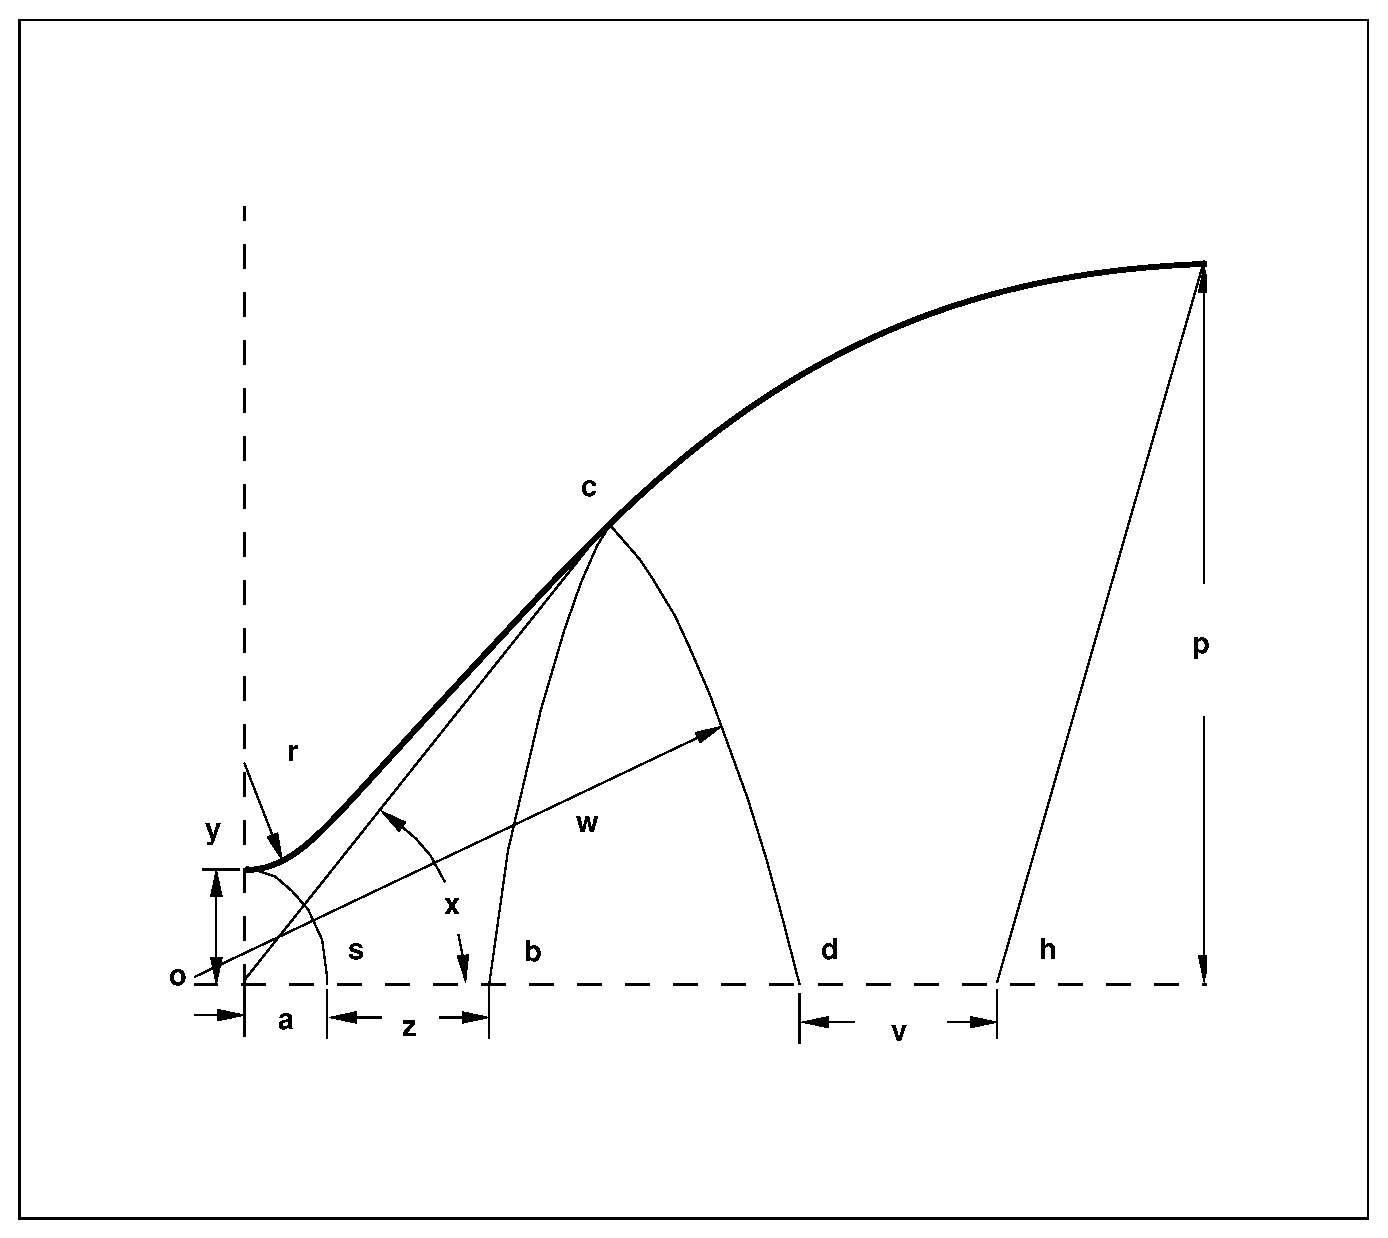
\includegraphics[width=13cm,height=7cm]{nozzle.eps}
\caption{Nomenclature for Nozzle Design}
\label{fig:nozzle}
\end{center}
\end{figure}

%----------------------------------------------------------------------------------------------------
\subsection{Inviscid Nozzle Design}

\begin{equation}
	\vec{q}\cdot\nabla(\frac{q^2}{2}) - a^2(\nabla \cdot \vec{q}) = 0 	
\label{eqn:gasdynq}
\end{equation}

	The \emph{gas dynamic equation} as shown above can be used as the starting point for developing 
the properties of a radial flow region (noting that $\vec{q}$ is the velocity vector, $q$ is the
magnitude of the velocity vector, and $a$ is the speed of sound).  In spherical co-ordinates
(which are the most convenient to use when considering a radial flow, since the flow travels outwards 
in all directions from a single source) the gradient of a vector can be expressed as,

\begin{equation}
	\nabla\cdot\vec{q} = \frac{1}{r^2}\frac{\partial}{\partial r}(r^2q_r) +
	\frac{1}{r \sin\theta}\frac{\partial}{\partial \theta}(q_{\theta}\sin\theta ) + 
	\frac{1}{r \sin\theta}\frac{\partial q_{\phi}}{\partial \phi}
\label{eqn:delq}
\end{equation}

	Applying the radial flow condition requires that the velocity in both angular 
directions be zero (i.e. $q_{\theta} = q_{\phi} = 0$) thus reducing the above operator to,

\begin{equation}
	\nabla\cdot\vec{q} = \frac{1}{r^2}\frac{d}{dr}(r^2q_r) = 
	\frac{dq}{dr} + 2\frac{q}{r}
\label{eqn:raddelq}
\end{equation}

	where $q_r = q$ since there is only velocity in one co-ordinate direction.

	The $\nabla$ operator on a scalar quantity in spherical co-ordinates can
be written as,

\begin{equation}
	\nabla q = \frac{\partial q}{\partial r} + \frac{1}{r}\frac{\partial q}{\partial \theta}
	+ \frac{1}{\sin \theta}\frac{\partial q}{\partial \phi}
\label{eqn:delscalq}
\end{equation}

	which after applying the radial flow constraints reduces to,

\begin{equation}
	\nabla q = \frac{dq}{dr} 
\label{eqn:raddelscalq}
\end{equation}

	Applying the results of Eqs. \ref{eqn:raddelq} and \ref{eqn:raddelscalq} to 
Eq. \ref{eqn:gasdynq} (and noting that $\vec{q} = q_r = q$ for radial flow) yields,

\begin{equation}
	\fbox{$
	(1 - M^2)\frac{dq}{dr} - 2\frac{q}{r} = 0
	$}
\label{eqn:radial}
\end{equation}

	This equation is the governing equation for inviscid radial flow. 

%---------------------------------------------------------------------------------------------

\subsubsection{Radial Flow Region}
	
	Starting with the fundamental radial flow equation derived in
Eq. \ref{eqn:radial} one can determine the relation between the Mach number at a given
location and the distance of this point from the radial flow source.  This is a key relationship
given that it is the Mach number distribution along the nozzle centreline 
(which is simply the radius along a particular ray from the 
radial flow source) that will be used to dictate the final nozzle contour.  The equations 
developed in this section apply between points B and D in Fig. \ref{fig:nozzle}  

	Starting by defining a non-dimensional velocity as,

\begin{equation}
	\fbox{$
	W = \frac{q}{a^*}
	$}
\label{eqn:w}
\end{equation}  
	
	where $a^*$ is the critical speed of sound (at M = 1), this non-dimensional
velocity can be related to the Mach number as follows.  Since $Ma = q$ and $Wa^*=q$ one can
write,

\begin{displaymath}
	(\frac{M}{W})^2 = (\frac{a^*}{a})^2
\end{displaymath}

	while from isentropic relations one can express the ratio of sound speeds as,

\begin{equation}
	(\frac{a^*}{a})^2 = \frac{2}{(\gamma + 1)}\Big\{1 + \frac{\gamma-1}{2}M^2\Big\} 
\label{eqn:isenaratio}
\end{equation}

	thus one can write,

\begin{displaymath}
	(\gamma+1)M^2 = W^2\Big\{2+(\gamma-1)M^2\Big\}
\end{displaymath}

	After isolating for $W^2$ and dividing through by $(\gamma -1)$, while defining $k$ as,

\begin{equation}
	\fbox{$
	k = \frac{\gamma+1}{\gamma-1}
	$}
\label{eqn:k}
\end{equation}
	
	one can rewrite the above expression as,

\begin{equation}
	\fbox{$
	W^2 = \frac{kM^2}{k-1 + M^2}
	$}
\label{eqn:wfromm}
\end{equation}

	Isolating $M^2$ in Eq. \ref{eqn:wfromm} yields an expression for the Mach number
from the non-dimensional velocity,

\begin{equation}
	\fbox{$
	M^2 = \frac{W^2(k-1)}{k-W^2}
	$}
\label{eqn:mfromw}
\end{equation}

	Going back to the governing equation for radial flow (Eq. \ref{eqn:radial}) 
and rearranging slightly,

\begin{displaymath}
	\frac{M^2-1}{2q} dq = \frac{1}{r} dr
\end{displaymath}
	
	one can use the definition of the non-dimensional velocity (Eq. \ref{eqn:w}) from which one can write
$dq = a^* dW$ and when combined with Eq. \ref{eqn:mfromw} allows the above relation to be expressed 
completely in terms of $W$.  Integrating the resulting expression from the sonic point (at which 
point $r = r_{cr}$ and $W = M = 1$) to some general point $r$ one obtains,

\begin{equation}
	\int_{r_{cr}}^{r}\frac{1}{r} dr = \frac{1}{2}\Big\{\int_{W=1}^{W}\frac{M^2}{W}dW - 
	\int_{W=1}^{W}\frac{1}{W}dW\Big\}
\label{eqn:rintraw}
\end{equation}

	Equation \ref{eqn:rintraw} can be integrated analytically if one assumes a perfect gas 
(hence $k$ is a constant with respect to the variable of integration $W$) by 
letting $x = W^2$ (and thus $\frac{1}{2}dx = W dW$),

\begin{displaymath}
	\ln(\frac{r}{r_{cr}}) = \frac{1}{2}\Big\{(k-1)\frac{1}{2}\int_{W=1}^{W}\frac{1}{k-x}dx
	- \ln(W)\vert_{W=1}^{W}\Big\}
\end{displaymath}

	Re-substituting back for $W$ and applying the limits yields,

\begin{displaymath}
	\ln(\frac{r}{r_{cr}}) = \ln\Big\{\frac{(k-W^2)^{\frac{1}{4}(1-k)}}{W^{\frac{1}{2}}
	(k-1)^{\frac{1}{4}(1-k)}}\Big\}
\end{displaymath}

	taking the exponential of both sides and defining a non-dimensional radius, $\overline{r}$,
as,

\begin{equation}
	\fbox{$
	\overline{r} = \frac{r}{r_{cr}}
	$}
\label{eqn:rbar}
\end{equation}

	yields,

\begin{displaymath}
	\overline{r} = \frac{(k-1)^{\frac{1}{4}(k-1)}}{W^{\frac{1}{2}}(k-W^2)^{\frac{1}{4}(k-1)}}
\end{displaymath}

	to phrase this result in a more usable form one can square both sides while
multiplying the right side by $W_k/W_k$, substituting for $M$ using Eq. \ref{eqn:mfromw}, 
and rearranging to get,

\begin{displaymath}
	\overline{r}^2 = \frac{M^k}{W^k}\frac{1}{M} = (\frac{M^2}{W^2})^{\frac{k}{2}}\frac{1}{M}
\end{displaymath}
	
	But from Eq. \ref{eqn:wfromm} one can express $W$ in terms of $M$ to yield,

\begin{equation}
	\fbox{$
	\overline{r}^2 = \frac{1}{M}\Big\{\frac{k-1+M^2}{k}\Big\}^{\frac{k}{2}}
	$}
\label{eqn:rbarfromm}
\end{equation}

	Equation \ref{eqn:rbarfromm} now gives us a means of determining the Mach number
vs. non-dimensional radius within the radial flow region of the nozzle.
Another key quantity in the radial flow region is the integrated angle, $\theta$, which for
radial flows can be shown to be equal to half the Prandtl-Meyer expansion angle for 2D flows.
This angle represents the angle through which a supersonic flow must be turned in order to be
accelerated from a Mach number of 1 to the given Mach number M, and can be expressed
for a perfect gas as,

\begin{equation}
	\fbox{$
	\theta = \frac{1}{2}\Big\{k^{\frac{1}{2}}\tan^{-1}\Big[\frac{M^2-1}{k}\Big]^{\frac{1}{2}}
	- \tan^{-1}(M^2-1)^{\frac{1}{2}}\Big\}
	$}
\label{eqn:intang}
\end{equation}

	This angle can be used to help determine the boundaries of the radial flow region, as
although Eq. \ref{eqn:rbarfromm} will yield a radial position for a given Mach number, the
Mach number at points D, C, and B are all unknown.  However, from the geometry of the nozzle
itself, it can be seen that the difference between the integrated angles
at points D and C must be equal to the physical angle COD in Fig. \ref{fig:nozzle} which is
the set maximum expansion angle $\omega$.  Therefore, if the Mach number at point D is known, then
so is the integrated angle at this point.  With this one can then fully determine point C
using the maximum expansion angle and Eq. \ref{eqn:intang} to get the Mach number at C, then
Eq. \ref{eqn:rbarfromm} to get the radial position of this point from the previously determined
$M_C$.  The same procedure can be used to find point B only in this case the difference 
between the integrated angles at points D and B is equal to twice the maximum expansion 
angle.  Thus, using Eqs. \ref{eqn:rbarfromm} and \ref{eqn:intang} one can fully determine
the Mach number distribution within the radial flow region provided the Mach number at point D
is known.

%---------------------------------------------------------------------------------------------

\subsubsection{Final Expansion Region}

	From the previous section, all that is required to fully describe the radial 
flow region is the Mach number at the end of this region, $M_D$.  However, from the
set nozzle parameters only the Mach number at point F is known since at this point
the flow has been accelerated to the exit Mach number.  Let the Mach number distribution 
between points D and F be described by a fifth order polynomial of the form,

\begin{equation}
	W = D_0 + D_1\xi + D_2\xi^2 + D_3\xi^3 + D_4\xi^4 + D_5\xi^5
\label{eqn:dpoly}
\end{equation}

	where along the axisymmetric axis,

\begin{displaymath}
	\xi = \frac{\overline{r}-\overline{r}_D}{\overline{X}_{DF}}
\end{displaymath}

	It should be noted that all the non-dimensional quantities above are non-dimensionalized
by the critical radius, as was done in Eq. \ref{eqn:rbar}.  In order to determine the 
co-efficients $D_0$ through $D_5$ one must make use of six boundary conditions.  Therefore,
specifying the velocity and its derivatives up to second order at each of the boundaries gives,

\begin{table}[!h]
\fontsizetable
\begin{center}
\begin{threeparttable}

\tablecaption{Non-Dimensional Boundary Conditions}

\begin{tabular}{ccccc}
\toprule
Point	& $\xi$	&	Velocity ($W$)		&	Acceleration ($W'$) 	&	Impulse ($W''$)\\
\midrule
D	& 0	&$W_D$	& $(\frac{dW}{d\overline{r}})_D = W'_D$ & $(\frac{d^2W}{d\overline{r}^2})_D = W''_D$\\
F	& 1	&$W_F$	& 0 & 0 \\
\bottomrule
\end{tabular}

%\begin{tablenotes}
%\end{tablenotes}

\label{table:dpoly}
\end{threeparttable}
\end{center}
\end{table}

	where it is noted that,

\begin{equation}
	\frac{dW}{d\xi} = D_1 + 2D_2\xi + 3D_3\xi^2 + 4D_4\xi^3 + 5D_5\xi^4
\label{eqn:dpolyfirst}
\end{equation}  

\begin{equation}
	\frac{d^2W}{d\xi ^2} = 2D_2 + 6D_3\xi + 12D_4\xi^2 + 20D_5\xi^3
\label{eqn:dpolysecond}
\end{equation}  

	At point D, since $\xi = 0$, applying the first boundary condition yields 
a direct solution for $D_0$,

\begin{equation}
	\fbox{$
	D_0 = W(0) = W_D 
	$}
\label{eqn:d0}
\end{equation}

	and similarly when applying the acceleration condition at point D one obtains $D_1$
(while noting that $d\xi X_{DF} = d\overline{r}$),

\begin{equation}
	\fbox{$
	D_1 = \frac{dW(0)}{d\xi} = \overline{X}_{DF}\frac{dW(0)}{d\overline{r}} = \overline{X}_{DF}W'_D
	$}
\label{eqn:d1}
\end{equation}

	Applying the last boundary condition at point D yields,

\begin{equation}
	\fbox{$
	D_2 = \frac{1}{2} \overline{X}_{DF}^2 W''_D
	$}
\label{eqn:d2}
\end{equation}

	Moving on to point F, skipping the velocity boundary condition for the moment
and applying the acceleration condition yields,

\begin{displaymath}
	D_4 = -\frac{1}{4}(D_1 + 2D_2 + 3D_3 + 5D_5)
\end{displaymath}

	Using the impulse condition at point F yields for $D_5$,

\begin{displaymath}
	D_5 = -\frac{1}{20}(2D_2 + 6D_3 + 12D_4)
\end{displaymath}

	which after using the previous result for $D_4$ gives,

\begin{displaymath}
	D_5 = \frac{1}{5}(3D_1 + 4D_2 + 3D_3)
\end{displaymath}

	Now using the velocity condition at F and isolating $D_3$ yields,

\begin{displaymath}
	D_3 = W_F - D_0 - D_1 - D_2 - D_4 - D_5	
\end{displaymath}	

	which when the results for $D_0, D_4,$ and $D_5$ are substituted 
results in,

\begin{equation}
	\fbox{$
	D_3 = 10(W_F - W_D) -6D_1 -3D_2
	$}
\label{eqn:d3}
\end{equation}

	Going back and replacing $D_3$ in the expressions for $D_4$ and $D_5$ 
yields,

\begin{equation}
	\fbox{$
	D_4 = -15(W_F - W_D) + 8D_1 + 3D_2
	$}
\label{eqn:d4}
\end{equation}

\begin{equation}
	\fbox{$
	D_5 = 6(W_F - W_D) - 3D_1  - D_2 
	$}
\label{eqn:d5}
\end{equation}

	At this point, it is noted that there are four apparent unknowns in the 
various co-efficients, $W_D, W_D', W_D''$, and $\overline{X}_{DF}$.  In order
to ensure a smooth increase in velocity along the axisymmetric axis between
points D and F, it can be assumed that $D_5 = 0$ which then allows for the
solution of $\overline{X}_{DF}$ from Eq. \ref{eqn:d5} as,

\begin{equation}
	\overline{X}_{DF} = -\frac{3W_D'}{W_D''}\Big\{1 - \sqrt{1 + \frac{4W_D''(W_F-W_D)}
	{3W_D'^2}}\Big\}
\label{eqn:xdf}
\end{equation}

	At this point we have reduced the number of unknowns to three, since the non-dimensional 
length $\overline{X}_{DF}$ is now a function of $W_D, W_D'$, and $W_D''$.  Since point
D is part of the radial flow region, the analytical expressions developed for this type of
flow can be used here as well.  Going back to Eq. \ref{eqn:rbarfromm} and using the relation
expressed in Eq. \ref{eqn:mfromw} one can obtain an equation for
$\overline{r}^2$ in terms of $W$,

\begin{equation}
	\fbox{$
	\overline{r}^2 = \frac{1}{W}\Big\{\frac{(k-1)}{(k-W^2)}\Big\}^{\frac{(k-1)}{2}}
	$}
\label{rbarfromw}
\end{equation}

	Taking the natural logarithm of both sides and differentiating yields
an expression for the first derivative of non-dimensional velocity
with respect to the non-dimensional radius,

\begin{equation}
	\frac{dW}{d\overline{r}}=\frac{2W(k-W^2)}{k(W^2-1)\overline{r}}=W'
\label{eqn:drdw}
\end{equation}
	
	The second derivative can also be found from Eq. \ref{eqn:drdw} and
be shown to be equal to,

\begin{equation}
	\frac{d^2W}{d\overline{r}^2}=\frac{-W'^2[3k-6W^2+(k+2)W^4]}{2W(k-W^2)(W^2-1)} = W''^2
\label{eqn:d2rdw2}
\end{equation}

	With Eqs. \ref{eqn:drdw} and \ref{eqn:d2rdw2} one can find the values of $W_D'$ and 
$W_D''$ from the value of $W_D$ alone, thus reducing the number of unknowns involved in determining
the desired polynomial co-efficients to one, namely $W_D$.  This was also the sole unknown required 
for the complete determination of the radial flow region.  To determine this value, one can
again make use of Eq. \ref{eqn:xdf} by noting that the value under the root must be positive to
ensure a real solution.  Therefore,

\begin{equation}
	(W_F - W_D)\geq-\frac{3}{4}\frac{W_D'^2}{W_D''}
\label{eqn:wdiff}
\end{equation}

	With this, one has a guide to selecting $W_D$, but the actual value must be chosen 
by the designer.  As a good first guess, $W_F - W_D$ can be taken as $1.5\%$ of $W_F$ and increased
until the criteria in Eq. \ref{eqn:wdiff} is satisfied.  Once $W_F - W_D$ is determined, $W_D$ can 
be used to completely determine the centreline Mach number distribution from the beginning 
of the radial flow region through to the nozzle exit inclusive.

%---------------------------------------------------------------------------------------------

\subsubsection{Initial Expansion Region}

	Having already established the Mach number distribution from the beginning of the
radial flow region (point B, Fig. \ref{fig:nozzle}) to the nozzle exit, the only region 
remaining to be defined is the initial expansion region near the nozzle throat (from
point A to B, Fig. \ref{fig:nozzle}).  Since the final expansion region was modeled using
a fourth order polynomial (recalling that the fifth co-efficient, $D_5$, was assumed zero),
for consistency, the initial expansion region will be treated similarly.  Thus one can write
for the segment along the axisymmetric axis between points A and B,

\begin{equation}
	W = C_0 + C_1\eta + C_2\eta^2 + C_3\eta^3 + C_4\eta^4
\label{eqn:cpoly}
\end{equation}

	where along the axis,

\begin{displaymath}
	\eta = \frac{\overline{r}-\overline{r}_A}{\overline{X}_{AB}}
\end{displaymath}

	As for the final expansion region, all the non-dimensional lengths are divided
by the critical radius (see Eq. \ref{eqn:rbar}).  In order to determine the 
co-efficients $C_0$ through $C_4$ one again has the option of applying six boundary conditions.  
Specifying the velocity and its derivatives up to second order at each of the boundaries
requires the derivatives of Eq. \ref{eqn:cpoly} up to second order while the boundary conditions
themselves are, 

\begin{table}[!h]
\fontsizetable
\begin{center}
\begin{threeparttable}

\caption{Non-Dimensional Boundary Conditions}

\begin{tabular}{ccccc}
\toprule
Point	& $\eta$&	Velocity ($W$)		&	Acceleration ($W'$) 	&	Impulse ($W''$)\\
\midrule
A	& 0&	1	& $(\frac{dW}{d\overline{r}})_A = W'_A$ & $(\frac{d^2W}{d\overline{r}^2})_A = W''_A$\\
B	& 1&	$W_B$	& $(\frac{dW}{d\overline{r}})_B = W'_B$ & $(\frac{d^2W}{d\overline{r}^2})_B = W''_B$\\
\bottomrule
\end{tabular}

%\begin{tablenotes}
%\end{tablenotes}

\label{table:cpoly}
\end{threeparttable}
\end{center}
\end{table}	

	Since the radial flow region includes point B, the non-dimensional velocity and position at point
B ($W_B$ and $\overline{r}_B$ respectively) are known quantities.  As well, Eqs. \ref{eqn:drdw} 
and \ref{eqn:d2rdw2} can both be used to determine $W'_B$ and $W''_B$ making the boundary conditions
at the end of the initial expansion region completely known.  However, at the beginning of this region the 
flow has just reached sonic speed, thus the nozzle throat region near point A is an area of transonic flow.  
This requires a specialized technique to solve, since one dimensional theory predicts a straight sonic
line at the exact geometric throat of the nozzle, whereas in real applications this line is curved
with the sonic point lying a finite distance downstream of the geometric throat (labeled $\epsilon$ in
Fig. \ref{fig:nozzle}) along the axisymmetric axis (Note: this line also \emph{starts} a finite distance 
upstream of the throat, but this region need not be considered in the present analysis).  There are several 
methods available to describe this transonic region (Sauer's Method, Hall's Method, Kliegel's Method) however
Kliegel's Method (which is a modified version of Hall's Method) will be used here.  

	In Kliegel's analysis
the non-dimensional velocity distribution along the axisymmetric axis in the throat region is 
given in the form of an equation in terms of $S$ (where $S = R + 1$).  In obtaining this solution, the 
throat region is assumed to be a circular arc of radius ($\rho_t$) while the parameter $R$ is the ratio of 
this radius to the half height, or radius, of the nozzle throat ($h$) thereby creating the relation 
$Rh = \rho_t$.  With the velocity distribution in this form one can obtain its derivatives for use in 
application to the boundary conditions, where at point A,

\begin{equation}
	(\frac{dW}{d\overline{r}})_A = \lambda R_1\Big\{1 - \frac{4\gamma-3}{24S} + \frac{652\gamma^2 
	+ 15\gamma + 333}{6912S^2}\Big\}
\label{eqn:waprime}
\end{equation}	

\begin{equation}
	(\frac{d^2W}{d\overline{r}^2})_A = (\lambda R_1)^2\Big\{1 - \frac{2\gamma}{3} + \frac{4\gamma^2 
	+ 69\gamma + 15}{96S}\Big\}
\label{eqn:wadprime}
\end{equation}

\begin{equation}
	(\frac{d^3W}{d\overline{r}^3})_A = (\lambda R_1)^3\Big\{\frac{4\gamma^2 - 57\gamma + 27}{24}\Big\}
\label{eqn:watprime}
\end{equation}	

	where $\lambda = \sqrt{\frac{2}{(\gamma+1)S}}$ and $R_1 = \frac{r_{cr}}{h}$.  
As well as yielding these derivatives Kliegel's analysis also yields the sonic point's distance 
downstream of the geometric nozzle throat ($\epsilon$) as,

\begin{equation}
	\overline{\epsilon}=\frac{\epsilon}{r_{cr}}=\frac{1}{4\lambda S}\Big\{1 - \frac{4\gamma -15}
	{72S} + \frac{412\gamma^2 + 270\gamma + 909}{10368S^2}\Big\}
\label{eqn:epsbar}
\end{equation}

	Therefore, if $S$ is known (which requires $R$ to be known) then the location of point
A can be determined from Eq. \ref{eqn:epsbar}.  However, the nozzle upper wall arc radius in the
throat region, $\rho_t$, cannot simply be assigned a value like a design variable, but must
be calculated based on further restrictions to be derived.  

	In a manner similar to that in the final expansion region, the boundary conditions can be 
applied to Eq. \ref{eqn:cpoly} to obtain the various co-efficients $C_O$ through $C_4$.  Starting with 
the boundary conditions at point A, through direct substitution (and noting that 
$d\eta X_{AB} = d\overline{r}$),

\begin{equation}
	\fbox{$
	C_0 = 1
	$}
\label{eqn:c0}
\end{equation}

\begin{equation}
	\fbox{$
	C_1 = \overline{X}_{AB}W'_A
	$}
\label{eqn:c1}
\end{equation}

\begin{equation}
	\fbox{$
	C_2 = \frac{1}{2}\overline{X}_{AB}^2W''_A
	$}
\label{eqn:c2}
\end{equation}

	Considering next the boundary conditions at point B, the velocity condition yields 
(while substituting for $C_0$),

\begin{displaymath}
	C_3 = (W_B - 1) - C_1 - C_2 - C_4
\end{displaymath}

	while the acceleration condition gives,

\begin{displaymath}
	C_3 = \frac{1}{3}(\overline{X}_{AB}W'_B - C_1 - 2C_2 - 4C_4)
\end{displaymath}

	Combining these two results yields for $C_4$,

\begin{equation}
	\fbox{$
	C_4 = -3(W_B -1) + W'_B\overline{X}_{AB} + 2C_1 + C_2
	$}
\label{eqn:c4}
\end{equation}

	and from back substitution one can get $C_3$ as,

\begin{equation}
	\fbox{$
	C_3 = 4(W_B -1) - W'_B\overline{X}_{AB} - 3C_1 - 2C_2
	$}
\label{eqn:c3}
\end{equation}

	At this point, one still has three unknowns, $W'_A$, $W''_A$ and $\overline{X}_{AB}$, 
in that although Eqs. \ref{eqn:waprime} and \ref{eqn:wadprime} can be used to find $W'_A$ and 
$W''_A$, the values of both $S$ and $R_1$ are needed to use these equations.  Therefore,
applying the remaining boundary condition at point B yields,

\begin{displaymath}
	\frac{d^2W(1)}{d\eta ^2} = \overline{X}_{AB}^2\frac{d^2W(1)}{d\overline{r}^2}
	= \overline{X}_{AB}^2 W''_B = 2C_2 + 6C_3 + 12C_4
\end{displaymath} 

	Using Eqs. \ref{eqn:c2}, \ref{eqn:c3} and \ref{eqn:c4} to replace $C_2$, $C_3$, and $C_4$ 
respectively yields a quadratic expression for $\overline{X}_{AB}$,

\begin{equation}
	(W''_A - W''_B)\overline{X}_{AB}^2 + 6(W'_A + W'_B)\overline{X}_{AB} - 12(W_B - 1)
\label{eqn:xabone}
\end{equation}

	This reduces $\overline{X}_{AB}$ to a function of both remaining unknowns, but one
is still left with finding values for $S$ and $R_1$.  However, in applying Kliegel's Method 
it is suggested that the second derivative of the nozzle contour in the region approximately
one diameter downstream of the geometric throat approximate the shape of a circle or hyperbola.
This criteria is best satisfied if the co-efficient $C_3$ is held equal to
the value $\frac{1}{6}W'''_A \overline{X}_{AB}^3$,

\begin{displaymath}
	C_3 = \frac{1}{6}W'''_A \overline{X}_{AB}^3 = 	4(W_B -1) - W'_B\overline{X}_{AB} - 3C_1 - 2C_2
\end{displaymath}

	which after using Eqs. \ref{eqn:c1} and \ref{eqn:c2} in the above yields,

\begin{equation}
	W'''_A \overline{X}_{AB}^3 + 6W''_A\overline{X}_{AB}^2 + 6(W'_B + 3W'_A)\overline{X}_{AB}
	-24(W_B -1) = 0 
\label{eqn:xabtwo}
\end{equation}

	Unfortunately this does not completely define the problem, as the determination of 
the derivatives at point A is still problematic in that the variables $S$ and $R_1$ are not
completely independent (as will be shown, $R_1$ depends on $S$).  However, Eqs. \ref{eqn:xabone} 
and \ref{eqn:xabtwo} can be used as a means of checking the accuracy of the values for $S$ 
and $R_1$ given that once $\overline{X}_{AB}$ is found using a particular set of $S$ and $R_1$ values,
one can then substitute this value and the corresponding derivative values into Eq. \ref{eqn:xabtwo} to 
check the result.  If Eq. \ref{eqn:xabtwo} is satisfied, a solution has been obtained.  

	Therefore, in order to determine the variables $S$ and $R_1$ (for use in finding the
derivative values at point A) one can make use of the parameter $K^2$, which is the ratio of the 
actual massflow passing through the nozzle throat (with a curved sonic line) to the massflow
passing through the nozzle assuming a straight sonic line (one dimensional flow).  From Kliegel's
Method this value can be expressed as,

\begin{equation}
	K^2 = 1 - \frac{\gamma-1}{96S^2}\Big\{1 - \frac{8\gamma -27}{24S} + 
	\frac{754\gamma^2 -757\gamma+3615}{2880S^2}\Big\}
\label{eqn:massflow}
\end{equation}

	while the ratio of critical radius to throat radius, $R_1$, can be expressed

\begin{equation}
	R_1 = \frac{r_{cr}}{h} = \frac{1}{2}K \csc(\frac{\omega}{2})
\label{eqn:r1}	
\end{equation}

	Equations \ref{eqn:massflow} and \ref{eqn:r1} provide the link between $S$ and $R_1$.
Similar to the final expansion region however, one is now forced to guess at a value for one of the 
required variables and then iterate slowly until all the criteria are met.  In this case, one
must first guess at a value of $S$ (or $R$ since $S = R + 1$).  With this, one can get a value
for $R_1$ from Eqs. \ref{eqn:massflow} and \ref{eqn:r1} and with these values one can then use 
Eqs. \ref{eqn:waprime},
\ref{eqn:wadprime}, and \ref{eqn:watprime} to get $W'_A$, $W''_A$, and $W'''_A$ which in turn
can be used in Eq. \ref{eqn:xabone} to find a value for $\overline{X}_{AB}$.  This value is 
then checked using Eq. \ref{eqn:xabtwo} and if this equation is not satisfied then the value
of $S$ can be changed until the convergence criteria is met.  Once $\overline{X}_{AB}$,  
$W'_A$, and $W''_A$ are determined, the co-efficients $C_0$ through $C_4$ can be found thereby
completely determining the Mach number distribution along the axisymmetric axis in the initial
expansion region.

	As a final note, since the nozzle contour is determined only at points along the 
characteristic mesh, the final velocity along the wall at the precise throat location cannot
be determined using the method of characteristics since the point closest to the nozzle throat
along the prescribed Mach number distribution is located a finite distance \emph{downstream} of the
geometric throat.  Therefore, making use of Kliegel's analysis once again, the throat wall
velocity can be expressed as,

\begin{equation}
	W_{throat} = 1 + \frac{1}{4S} - \frac{14\gamma - 57}{288 S^2} + \frac{2364\gamma^2 - 3915\gamma + 14337}
	{82944S^3}
\label{eqn:uwall}
\end{equation}
	

%---------------------------------------------------------------------------------------------

\subsubsection{Nozzle Wall Determination}

	With the desired Mach number distribution established and the final Mach
line originating from point F, one has everything required to use the two-dimensional
method of characteristics to determine the flowfield within the diverging section of the nozzle.  
However, what is still 
lacking is a means of knowing when to stop marching the characteristics in the direction 
perpendicular to the nozzle axis.  This is of critical importance as this stopping point
determines the upper wall of the nozzle, which is the desired quantity.  Therefore,
going back to the radial flow region, one can make use of the stream function, $\psi$,
and determine its value at the nozzle boundary.  
	
	Since the difference between stream
functions at any two points within a flow is equal to the mass flow between the streamlines
on which the stream functions are taken, if one knows the stream function value on the
nozzle axis, plus the value at \emph{ANY} point on the nozzle wall, then this difference
must be constant given that the the mass flow through the nozzle is constant (or from another
viewpoint, since the flow must follow the contour of the nozzle wall, the wall itself is
a streamline.  Knowing the value of the stream function at a single point along a streamline yields 
the value along all points of the streamline, thus finding the nozzle contour is equivalent
to finding a streamline with a specific stream function value).

  	Using the properties of radial flow, considering an incremental area on a sphere of 
radius $r$ bounded by the angles $\alpha$ and $\alpha + d\alpha$ one can write the differential 
stream function as

\begin{equation}
	d\psi = \rho q (\pi r^2 \sin \alpha d\alpha)
\label{eqn:diffstream}
\end{equation}

	Integrating Eq. \ref{eqn:diffstream} from the nozzle axis to some angle $\alpha$,

\begin{displaymath}
	\int_{\alpha=0}^{\alpha}d\psi = \rho q \pi r^2\int_{\alpha=0}^{\alpha}\sin \alpha d\alpha = 
	\psi = -\rho q \pi r^2 \cos \alpha \vert_0^{\alpha}
\end{displaymath}

	Therefore one can write,

\begin{equation}
	\psi = \rho q \pi r^2 (1-\cos\alpha)
\label{eqn:psi}
\end{equation}	

	where $\alpha$ is a physical angle between the axisymmetric axis, the origin of the
radial flow zone, and some point above the axis (which is not to be confused with the integrated
angle $\theta$ in Eq. \ref{eqn:intang}).  Non-dimensionalizing this value by the critical
radius $r_{cr}$, the sonic sound speed $a^*$, the total density (found from the nozzle
chamber conditions) $\rho_o$, and $\pi$ yields,

\begin{equation}
	\fbox{$
	\overline{\psi} = \overline{\rho} W \overline{r}^2 (1-\cos\alpha)
	$}
\label{eqn:psibar}
\end{equation}	
	
	where $\overline{\rho} = \frac{\rho}{\rho_o}$.  Since point C lies within the
radial flow region, Eq. \ref{eqn:psibar} applies here.  Further, the physical angle $\alpha$ at point
C is known since this is also the location of the maximum expansion angle, $\omega$.  For isentropic flow 
the density ratio is a function of Mach number alone (and $\gamma$, but this is a property of 
the fluid, not the flow), which in turn is dependent only on $W$ within the radial flow region (see 
Eq. \ref{eqn:mfromw}).
Therefore, with the centreline Mach number distribution (which yields $W_C$ and $\overline{r}_C$)
one has all the information required to determine the value of the non-dimensional stream 
function at point C, which is a constant along the nozzle wall.  

	With the value of the stream function at the nozzle wall fixed, all that remains
is to calculate the incremental stream function at each intersection point when applying the 
method of characteristics.  To do this, one requires the differential of the non-dimensional stream 
function with respect to a change in height above the axisymmetric axis (i.e. $\frac{d\overline{\psi}}
{d\overline{y}}$).  When the incremental change in $\overline{y}$ is small then a good approximation for 
$d\overline{\psi}$ (given by Evvard) is,

\begin{equation}
	\int_{A}^{B}d\overline{\psi} = \overline{\psi}_B - \overline{\psi}_A = 
	\Big\{(\frac{\overline{\rho}W}{4M\sin(\mu + \theta_f)})_A + (\frac{\overline{\rho}W}
	{4M\sin(\mu + \theta_f)})_B \Big\}(\overline{y}^2_B - \overline{y}^2_A)
\label{eqn:dpsibar}
\end{equation}
	
	where $\mu$ is the Mach angle ($\sin^{-1}[1/M]$), $\theta_f$ here is the flow angle
($\tan^{-1}[v/u]$), and $\overline{y}$ is the perpendicular distance from the axisymmetric 
axis divided by the critical radius ($y/r_{cr}$).
 
	In most cases, the intersection of two characteristics will not occur at the exact location
of the nozzle wall (i.e. the value of the stream function will be slightly higher than the wall value
at the final intersection) and hence an interpolation procedure must be used to determine the 
distance from the axisymmetric axis at which the stream function reaches the correct value ($\overline{\psi}_C$).  
The percentage of the last increment (in the direction normal to the axis) to be applied is calculated as,

\begin{equation}
	\beta=\frac{\overline{\psi}_c - \overline{\psi}_{j-1}}{\overline{\psi}_j - \overline{\psi}_{j-1}}
\label{eqn:percent}
\end{equation}

	where $j$ increases as one travels away from the axis.  Since $\overline{y}^2$ is proportional to 
$d\overline{\psi}$
(as can be seen in Eq. \ref{eqn:dpsibar}) the nozzle wall height is determined using,

\begin{equation}
	\overline{y}_{wall}^2 = \overline{y}_{j-1}^2 + \beta(\overline{y}_j^2 - \overline{y}_{j-1}^2)
\label{eqn:ywall}
\end{equation}

	while the remaining quantities of interest at the nozzle wall are found using,

\begin{displaymath}
	\overline{x}_{wall}=\overline{x}_{j-1} + \beta(\overline{x}_j-\overline{x}_{j-1})
\end{displaymath}

\begin{displaymath}
	q_{wall}=q_{j-1} + \beta(q_j-q_{j-1})
\end{displaymath}

\begin{displaymath}
	\theta_{wall}=\theta_{j-1} + \beta(\theta_j-\theta_{j-1})
\end{displaymath}
	
	where again, $\theta_j$ is the flow angle, \emph{NOT} the integrated angle from Eq. \ref{eqn:intang}.
%---------------------------------------------------------------------------------------------

\subsubsection{Dimensionalizing Nozzle Wall Co-Ordinates}

	Having applied the two dimensional method of characteristics and determined the nozzle shape
in terms of non-dimensional co-ordinates, all that remains is to calculate the physical co-ordinates.
To do this one requires the value of $r_{cr}$ which was used to non-dimensionalize all the length
variables.  

	Considering the mass flow through the nozzle ($\dot{m}$), this quantity can be
expressed as twice the value of the non-dimensional stream function at point C 
(i.e. $2\overline{\psi}_C$) since 
$\overline{\psi}_C$ is calculated for the upper portion of the axisymmetric nozzle only (from $\alpha = 0$ to 
$\omega$), thus using Eq. \ref{eqn:psibar}

\begin{displaymath}
	\dot{m}=2\overline{\psi}_C=2\overline{\rho}_C W_C \overline{r}^2_C (1-\cos\omega)
\end{displaymath}

	However, at the nozzle exit the mass flow can be expressed as,

\begin{equation}
	\dot{m}=\rho_Fu_F(\pi h_{exit}^2)
\label{eqn:massflowexit}
\end{equation}

	since the flow is parallel to the axis at the exit (therefore $v = 0$) and
the exit area is circular.  Non-dimensionalizing the above expression in the same
fashion as was done for $\overline{\psi}$ (thus dividing by $\rho_o$, $a^*$, $\pi$, and 
$r_{cr}$) and equating the two expressions for $\dot{m}$ yields,

\begin{equation}
	\fbox{$
	\overline{h}_{exit}^2=\frac{2\overline{\psi}_C}{\overline{\rho}_F W_F}
	$}
\label{eqn:hexitbar}
\end{equation}

	Assuming a one dimensional nozzle with a straight sonic line located at the geometric throat,
one can express the mass flow rate through this idealized nozzle as,
	
\begin{equation}
	\dot{m}_{1D} = \rho^* a^* (\pi h^2)
\label{eqn:massflow1D}
\end{equation}
	
	Recalling the analysis used in the throat region of the nozzle, Eq. \ref{eqn:massflow}
yields the ratio of the actual mass flow through the nozzle to the massflow of a one-dimensional
nozzle.  Rewriting Eq. \ref{eqn:massflow} here for convenience,

\begin{displaymath}
	K^2 = 1 - \frac{\gamma-1}{96S^2}\Big\{1 - \frac{8\gamma -27}{24S} + 
	\frac{754\gamma^2 -757\gamma+3615}{2880S^2}\Big\}
\end{displaymath}

	one can also calculate this parameter using the ratio of Eq. \ref{eqn:massflowexit} 
to Eq. \ref{eqn:massflow1D},

\begin{displaymath}
	\frac{\dot{m}}{\dot{m}_{1D}}=\frac{\rho_F u_F \pi h_{exit}^2}{\rho^* a^* \pi h^2}=
	\frac{\overline{\rho}_F W_F \overline{h}_{exit}^2}{\overline{\rho}^*\overline{h}^2}=K^2
\end{displaymath}

	which allows an expression for $\overline{h}^2$ to be written as,

\begin{equation}
	\fbox{$
	\overline{h}^2 = \frac{\overline{\rho}_F W_F \overline{h}_{exit}^2}{K^2 \overline{\rho}^*}
	$}
\label{eqn:hbar}
\end{equation}	

	Using Eq. \ref{eqn:hexitbar} to find $\overline{h}_{exit}$ and then Eq. \ref{eqn:hbar} to find
$\overline{h}$, one can then find $r_{cr}$ from the definition of $\overline{h}$,

\begin{equation}
	\overline{h}=\frac{h}{r_{cr}}
\label{eqn:rcr}
\end{equation}

%----------------------------------------------------------------------------------------------
\subsection{Viscous Nozzle Design}

	The previous section details the procedure for designing an axisymmetric nozzle 
in the absence of a boundary layer.  However,
in practice a nozzle created using this design procedure will in fact have a turbulent
boundary layer over the majority of its length.  Therefore, a method is required to adjust the
inviscid nozzle contour to account for the presence of the boundary layer.  One such method
is that of Edenfield, where experimental correlations are used to determine the mass flow deficit, or 
displacement thickness ($\delta^*$), of the boundary layer which is then related to a shift ($\Delta y$) of
the nozzle contour in a direction normal to the axis.  Since the displacement thickness is simply the 
height of a region of flow (at the freestream density and velocity) that when added to the actual mass
flow (including boundary layer effects, i.e., slower moving flow near the surface) would equal the 
theoretical massflow through the inviscid contour in the absence of a boundary layer, one can use this value 
to adjust the nozzle shape to maintain the inviscid mass flow value.  However, since $\delta^*$ is 
calculated normal to the nozzle surface 
(which has a slope $\theta_{wall}$) while $\Delta y$ is normal to the axisymmetric axis, a small
correction needs to be applied.  Considering the mass flow deficit (per unit depth) calculated from the
displacement thickness,

\begin{displaymath}
	\Delta \dot{m} = \rho q \delta^*
\end{displaymath}
	
	while if the nozzle correction height is used,

\begin{displaymath}
	\Delta \dot{m} = \rho u \Delta y
\end{displaymath}

	where here $u$ is used instead of $q$ as $\Delta y$ is parallel to the velocity
component $v$.  Noting that $u = q\cos\theta_{wall}$ and making the mass flow deficit equal as calculated
from either height yields,

\begin{equation}
	\fbox{$
	\Delta y = \frac{\delta^*}{\cos\theta_{wall}}
	$}
\label{eqn:deltay}
\end{equation}

  If the upper wall is increased in height by an amount equal to $\Delta y$ then the nozzle contour 
accounting for viscosity can be written as,

\begin{equation}
	y_{viscous} = y_{inviscid} + \Delta y = y_{inviscid} + \frac{\delta^*}{\cos\theta_{wall}}
\label{eqn:yvis}
\end{equation}

	In order to calculate the displacement thickness, Edenfield suggests the relation,

\begin{equation}
	\delta^* = \frac{21}{50}\frac{x}{Re_{ref}^{0.2775}} 
\label{eqn:dispthick}
\end{equation}	

	where $x$ is the physical location downstream as measured from the nozzle throat while the 
reference Reynolds number is defined as,

\begin{equation}
	Re_{ref}=\frac{\rho_{ref}q_{inv}x}{\mu_{ref}}
\label{eqn:reyref}
\end{equation}

	where $q_{inv}$ is the velocity calculated from the inviscid profile at the given $x$ location,
while $\rho_{ref}$ and $\mu_{ref}$ are calculated at the reference temperature and the freestream pressure
(which is the pressure at the $x$ location assuming no viscosity).  The reference temperature is
found from the reference enthalpy, $h_{ref}$, defined as,

\begin{equation}
	h_{ref}=\frac{1}{2}(h_{wall} + h_{inv}) + \frac{11}{50}(h_{aw} - h_{inv})
\label{eqn:href}
\end{equation}


	where $h_{wall}$ is the specific enthalpy calculated at the specified wall temperature, $h_{aw}$ is
the specific adiabatic wall enthalpy, and $h_{inv}$ is the specific enthalpy calculated from the
inviscid contour at the given $x$ location,

\begin{equation}
	h_{inv}=h_{tot} - \frac{1}{2}q_{inv}^2
\label{eqn:hinv}
\end{equation}

	To calculate the specific adiabatic wall enthalpy Edenfield uses (for turbulent boundary layers),

\begin{equation}
	h_{aw} = h_{inv} + \frac{9}{10}(h_{tot} - h_{inv})
\label{eqn:haw}
\end{equation}

	With Eqs. \ref{eqn:yvis} - \ref{eqn:haw} one has all the information required to adjust the
inviscid contour to account for the presence of a turbulent boundary layer.  To calculate the boundary
layer thickness itself, $\delta_{bound}$, the following relations can be applied,

\begin{equation}
	\delta_{bound}=\frac{11}{10}x(\frac{\frac{39}{200}M_{inv}^{\frac{3}{8}}}{Re_{x}^{\frac{83}{500}}})
\label{eqn:deltab}
\end{equation}

	where 

\begin{equation}
	Re_x=\frac{\rho_{inv}q_{inv}x}{\mu_{inv}}
\label{eqn:reyx}
\end{equation}

	and finally,

\begin{equation}
	y_{bound}=y_{vis} - \frac{\delta_{bound}}{\cos\theta_{wall}}
\label{eqn:ybound}
\end{equation}

%----------------------------------------------------------------------------------------------
\subsection{Subsonic Nozzle Contour}

	Although the design of the nozzle has been detailed in full from the throat to 
the exit, one may wish to add a subsonic portion upstream of the throat.  Since uniform
flow is desired at the throat, a contoured upper wall can be used to
produce the desired results.  One example of such an axisymmetric contour is,

\begin{equation}
	h_{wall} = \frac{h_{throat}}{ \sqrt{1 - \Big\{1- (\frac{h_{throat}}{h_{chamber}})^2\Big\}
	\frac{(1-\frac{x^2}{l^2})^2}{1+(\frac{x^2}{3l^2})^3} }}
\label{eqn:subsonic}
\end{equation}
	
	where $l$ is the distance between the combustion chamber exit and the nozzle throat (which can be 
taken as a percentage of the length of the diverging portion of the nozzle) while
$x$ is the distance of the location under consideration as measured from the combustion chamber exit.  
The value of $h_{chamber}$ can be determined from the isentropic relation for areas in a 
converging/diverging duct (remembering that for an axisymmetric nozzle, the area is proportional to the
\emph{square} of the radius, or nozzle half height $h$),

\begin{equation}
	(\frac{h_{chamber}}{h_{throat}})^2 = \frac{A}{A^*} = \frac{1}{M_{chamber}}\Big\{(\frac{2}{\gamma +1})
	(1 + \frac{\gamma-1}{2}M_{chamber}^2)\Big\}^\frac{\gamma +1}{2(\gamma -1)} 
\label{eqn:area}
\end{equation}

	and the assumption of a negligible velocity exiting the combustion chamber (e.g. 
$M_{chamber} = 0.1$).

%--------------------------------------------------------------------------------------------------
\section{Results}

\subsection{Kerosene/Air Combustion}

	The combustion of kerosene with air can be written as follows,

\begin{equation}
	\phi C_{12}H_{24} + 18 (O_2 + 3.76 N_2) \longrightarrow 12 H_2O + 12 CO_2 + 67.68 N_2
\label{eqn:kerocombair}
\end{equation}

	where air is treated on a kmol basis to be composed of $21\% O_2$ and $79\% N_2$ (and 
the nitrogen is treated as inert during the combustion process).  The 
fuel to air ratio on a mass basis requires a knowledge of the molecular weight of air.  However, one must
be careful to make a distinction between a \emph{kmol of air} and a kmol of an individual species, since air
is actually a composite species of two more basic species (oxygen and nitrogen).  Thus on a kmol basis this
value can be calculated as 28.8503 $kg_{air}$/kmol, or, since one kmol of air actually contains 
4.76 kmols of primary species (i.e. 4.76 kmol/$kmol_{air}$) then molecular weight of air per 
\emph{kmol of air} is actually 4.76 x 28.8503 = 137.3274 $kg_{air}/kmol_{air}$.

	Therefore from Eq. \ref{eqn:kerocombair} for every 1 kmol of fuel there are 18 kmols of air, which
is actually 18 x 4.76 = 85.68 kmols, and thus the stoichiometric fuel to air ratio on a molar basis is
$(\frac{f}{a})_{st}$ 1/85.68 or 0.01167.  On a mass basis using the molecular weight calculated above
for air of 28.8503 kg/kmol and a molecular weight for kerosene of 168.32256 kg/kmol ($C_{12}H_{24}$) one 
obtains $(\frac{f}{a})_{st}$ = 0.06809. 

	Applying the Gibbs Minimization Technique and solving for the nineteen species shown in 
Table \ref{table:spmapair} yields the equilibrium composition shown in 
Fig. \ref{fig:kero_air}(B) (where the equivalence ratio is unity and an initial temperature and 
pressure of 300 K and 1.5 MPa respectively are used).	

\begin{figure}[hb]
\begin{center}
\begin{subfigure}[]{
\psfrag{y}[c][c][0.7][0]{Temperature [K]}
\psfrag{z}[c][c][0.7][0]{$\gamma$}
\psfrag{x}[c][c][0.7][0]{Equivalence Ratio}
\psfrag{a}[l][l][0.45][0]{Equilibrium Temperature}
\psfrag{b}[l][l][0.45][0]{Throat Temperature}
\psfrag{c}[l][l][0.45][0]{$\gamma$}
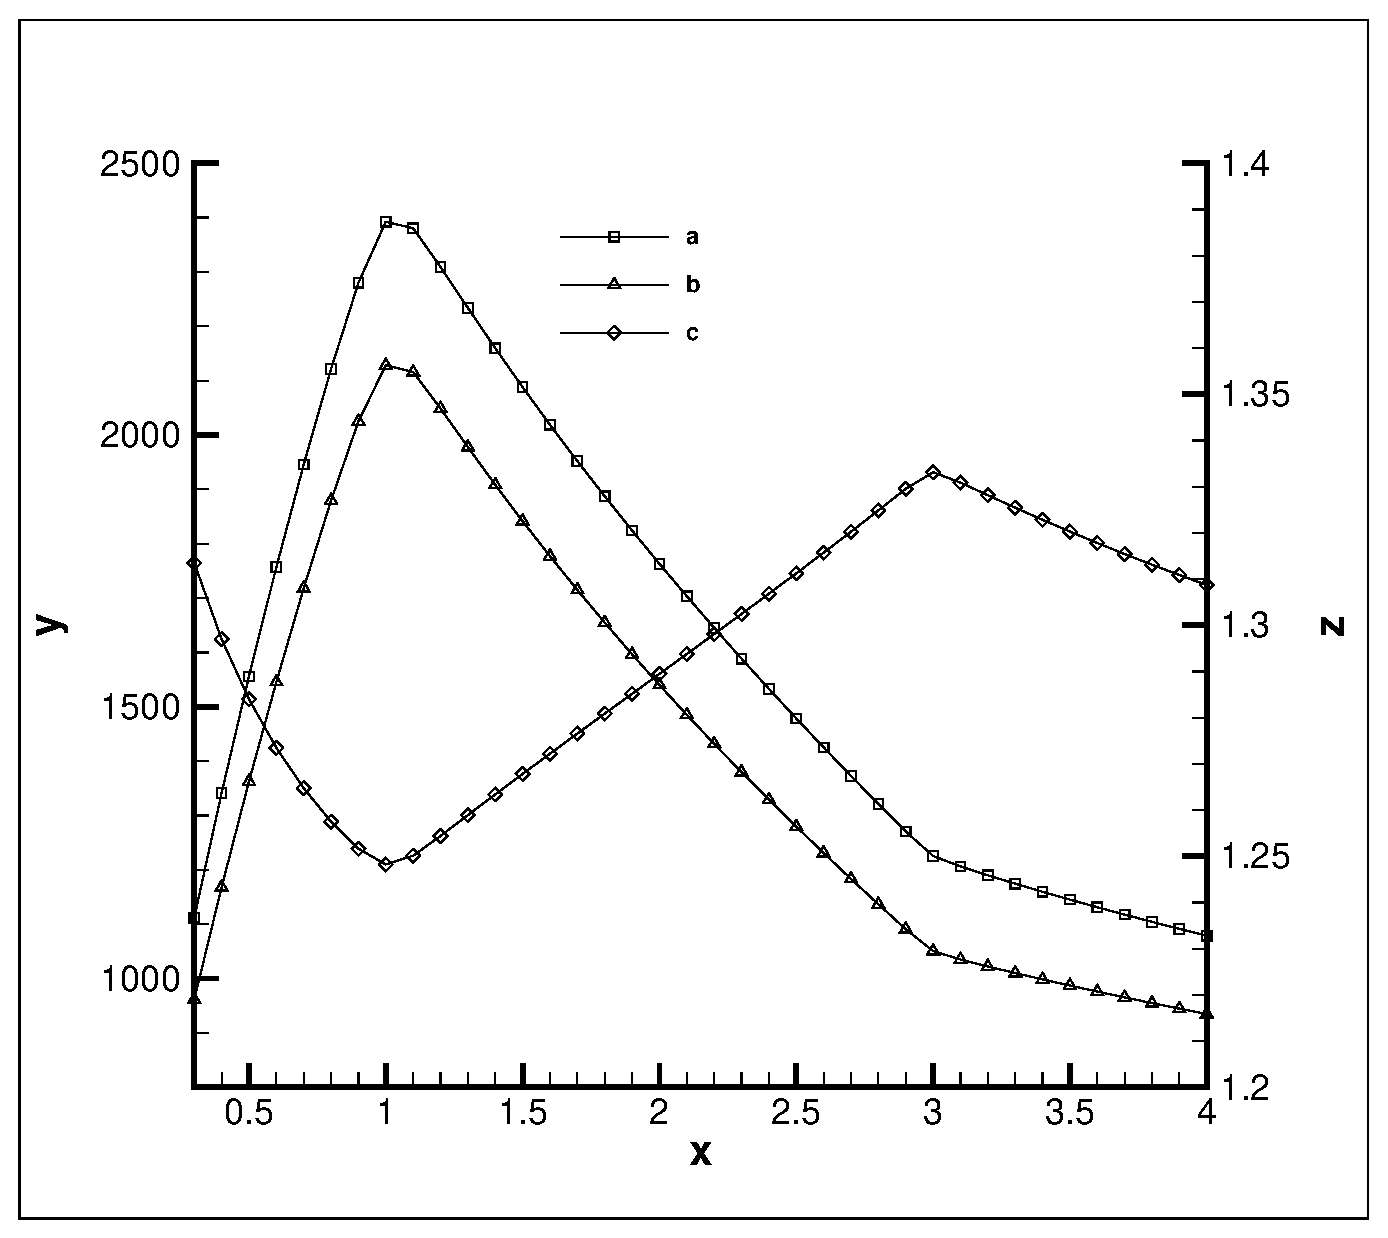
\includegraphics[width=7cm]{kero_air_tempvsphi.eps}}
\end{subfigure}
\begin{subfigure}[]{
\psfrag{y}[c][c][0.7][0]{Mass Fraction ($c_i$)}
\psfrag{x}[c][c][0.7][0]{Species}
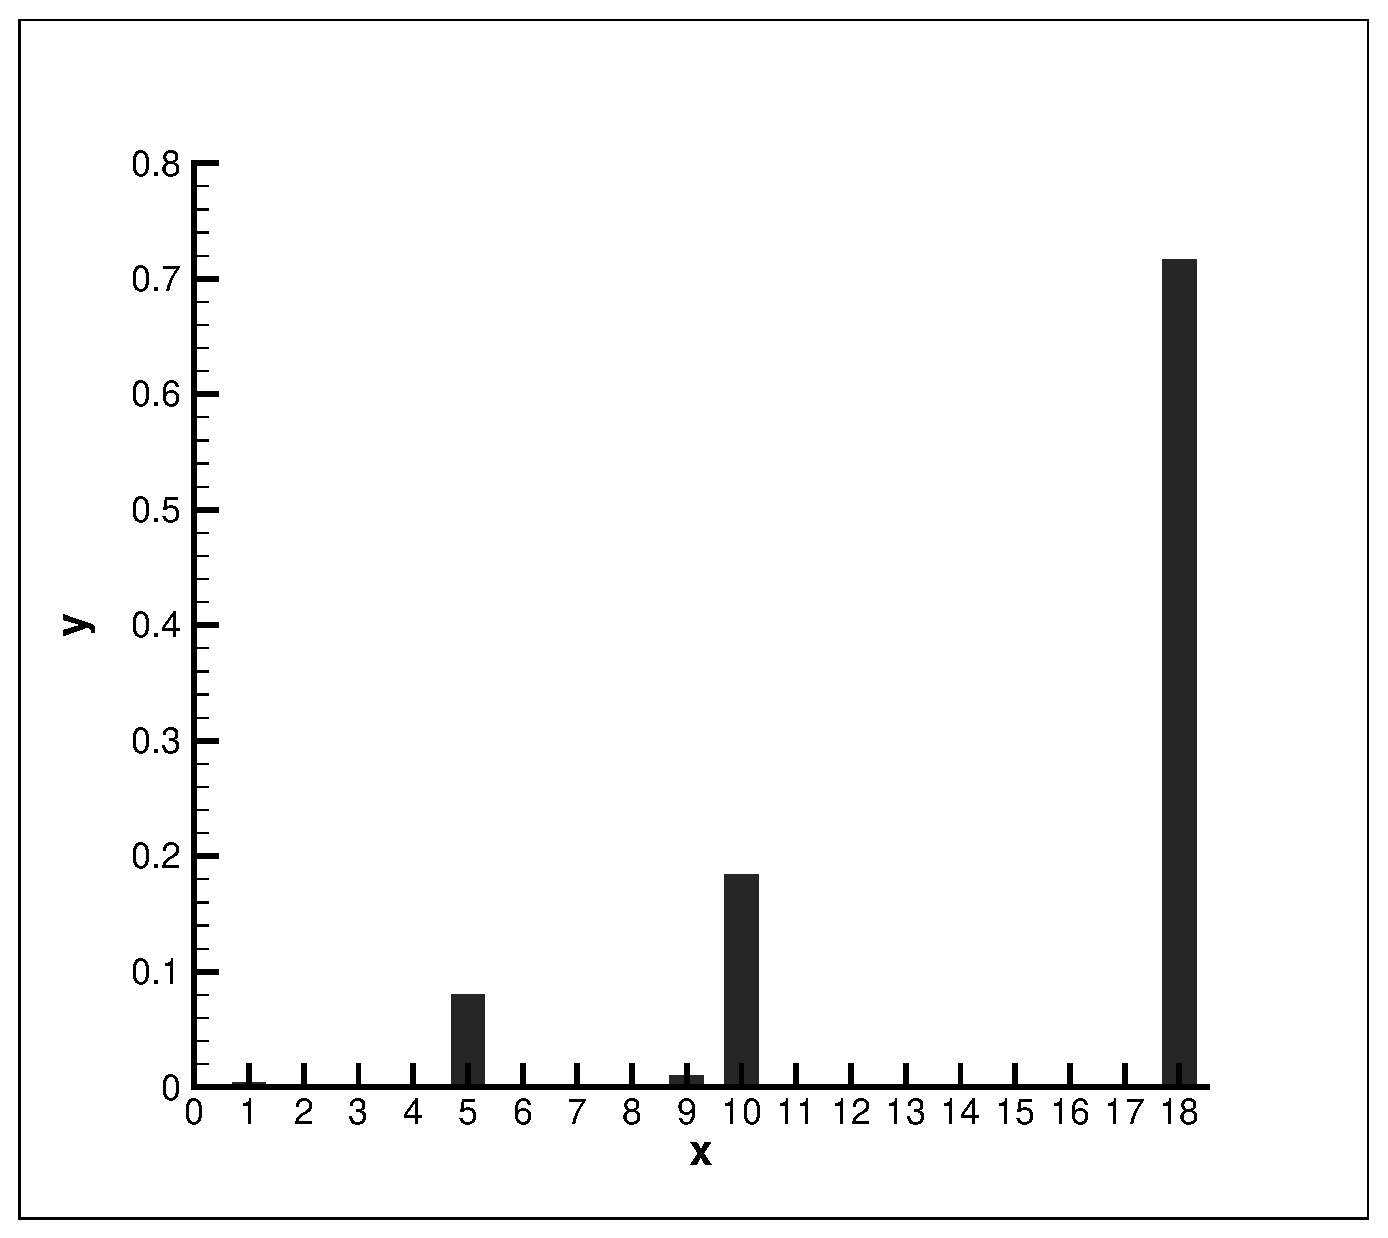
\includegraphics[width=7cm]{kero_air_mass_phi1.eps}}
\end{subfigure}
% One can specify [angle=x,width=y,height=z] for the graphics
\caption{Equilibrium combustion results for (A) variable equivalence ratio and (B) equivalence ratio
of 1 (stoichiometric combustion)}
\label{fig:kero_air}
\end{center}
\end{figure}



\begin{table}[h]
\fontsizetable\begin{center}
\begin{threeparttable}

\tablecaption{Species Map for Figure \ref{fig:kero_air}}

\begin{tabular}{ccccccccccccccccc}
\toprule
0 & 1 & 2 & 3 & 4 & 5 & 6 & 7 & 8 & 9\\
\midrule
$H_2$ & $O_2$ & $H$ & $O$ & $OH$ & $H_2O$ & $HO_2$ & $C_2H_2$ & $C_2H_4$ & $CO$ \\ 

\midrule
10 & 11 & 12 & 13 & 14 & 15 & 16 & 17 & 18\\
\midrule
$CO_2$ & $CH_3$ & $CH_4$ & $H_2CO$ & $C_6H_{12}O$ & $C_{12}H_{24}$ & $N$ & $NO$ & $N_2$\\
\bottomrule
\end{tabular}

%\begin{tablenotes}
%\end{tablenotes}

\label{table:spmapair}
\end{threeparttable}
\end{center}
\end{table}

	One can see from Fig. \ref{fig:kero_air}(A) that as the fuel to air ratio is raised from 
fuel lean conditions (low $\phi$) to 
a $\phi$ of approximately 1, the equilibrium combustion temperature rises reaching
a peak of approximately 2400 K (which assuming isentropic expansion yields a peak throat temperature
of approximately 2100 K).  At stoichiometric conditions, the complete combustion mass fractions of each species
can be determined directly from Eq. \ref{eqn:kerocombair} by multiplying the number of kmols of each
species by its molecular weight and dividing by the total mass of either the products or reactants 
(as mass is conserved during the combustion process).  By doing this one finds that the mass fraction
of water ($H_2O$, species 5) is approximately 0.082 while that of carbon dioxide ($CO_2$, species 10) is
approximately 0.200.  Both of these values are far less than the stoichiometric mass fraction of
nitrogen ($N_2$, species 18) of 0.718.  Comparing these values with those shown in Fig. \ref{fig:kero_air}(B)
one can see that the Gibbs Minimization Technique, which although based on the assumption of chemical 
equilibrium and not complete combustion, appears very accurate in that it matches the complete combustion
solution closely.  This would indicate that the complete combustion model in Eq. \ref{eqn:kerocombair}
is an accurate model of the combustion process in this case.


%----------------------------------------------------------------------------------------------------------
\subsection{Kerosene/Pure Oxygen Combustion}

	The complete combustion reaction for the combustion of kerosene ($C_{12}H_{24}$) with
pure diatomic oxygen ($O_2$) (which would be the case in a kerosene rocket chamber) can be written as follows,

\begin{equation}
	\phi C_{12}H_{24} + 18 O_2 \longrightarrow 12 H_2O + 12 CO_2
\label{eqn:kerocombo2}
\end{equation}

	which on a molar basis yields a fuel to air ratio, $(\frac{f}{a})_{st}$, of 1/18 or 0.05556.  Using 
molecular weights of 168.32256 kg/kmol and 31.9988 kg/kmol for kerosene and oxygen respectively 
yields a $(\frac{f}{a})_{st} = 0.2916$ on a mass basis.  Applying the Gibbs Minimization Technique 
(using sixteen species in this case as there are no species containing nitrogen) yields
the equilibrium composition shown in Fig. \ref{fig:kero_oxy}(B) with initial temperature and pressure
of 300 K and 1.5 MPa respectively.

\begin{figure}[h]
\begin{center}
\begin{subfigure}[]{
\psfrag{y}[c][c][0.7][0]{Temperature [K]}
\psfrag{z}[c][c][0.7][0]{$\gamma$}
\psfrag{x}[c][c][0.7][0]{Equivalence Ratio}
\psfrag{a}[l][l][0.45][0]{Equilibrium Temperature}
\psfrag{b}[l][l][0.45][0]{Throat Temperature}
\psfrag{c}[l][l][0.45][0]{$\gamma$}
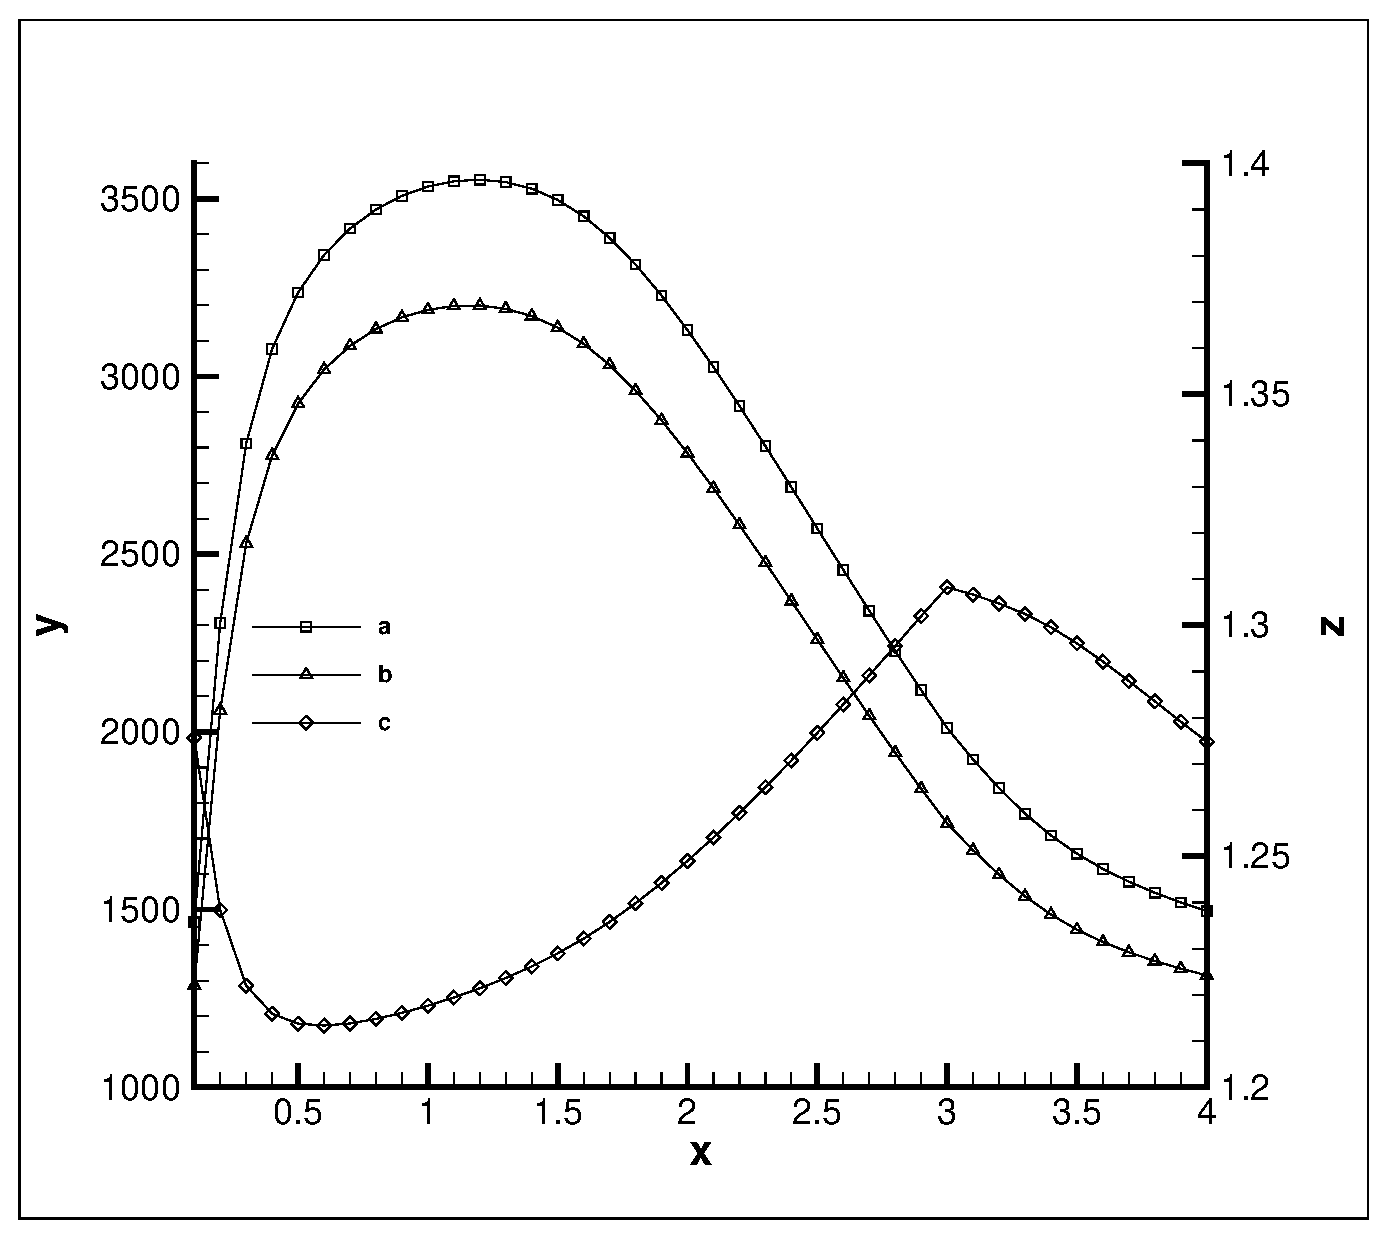
\includegraphics[width=7cm]{kero_oxy_tempvsphi.eps}}
\end{subfigure}
\begin{subfigure}[]{
\psfrag{y}[c][c][0.7][0]{Mass Fraction ($c_i$)}
\psfrag{x}[c][c][0.7][0]{Species}
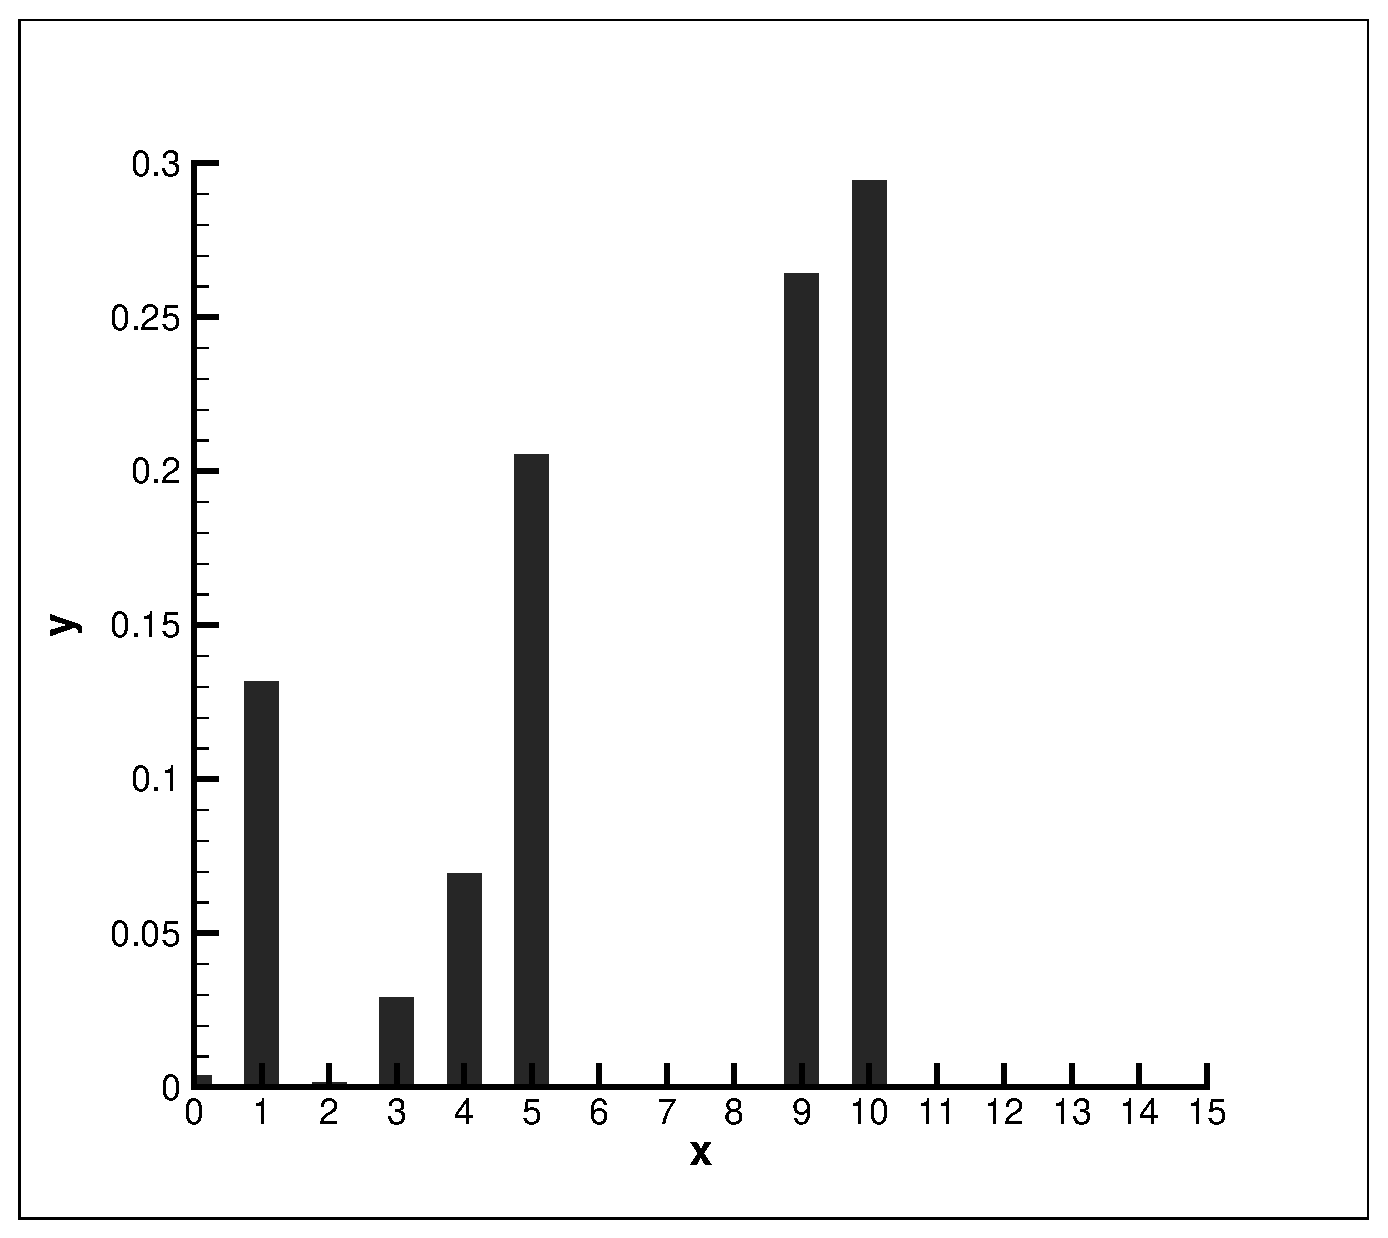
\includegraphics[width=7cm]{kero_oxy_phi1.eps}}
\end{subfigure}
% One can specify [angle=x,width=y,height=z] for the graphics
\caption{Equilibrium combustion results for (A) variable equivalence ratio and (B) equivalence ratio
of 1 (stoichiometric combustion)}
\label{fig:kero_oxy}
\end{center}
\end{figure}

\begin{table}[h]
\fontsizetable
\begin{center}
\begin{threeparttable}

\tablecaption{Species Map for Figure \ref{fig:kero_oxy} and Figure \ref{fig:kero_oxy_multiphi}}

\begin{tabular}{cccccccccccccccc}
\toprule
0 & 1 & 2 & 3 & 4 & 5 & 6 & 7 & 8\\
\midrule
$H_2$ & $O_2$ & $H$ & $O$ & $OH$ & $H_2O$ & $HO_2$ & $C_2H_2$ & $C_2H_4$\\ 

\midrule
9 & 10 & 11 & 12 & 13 & 14 & 15 & \\
\midrule
$CO$ & $CO_2$ & $CH_3$ & $CH_4$ & $H_2CO$ & $C_6H_{12}O$ & $C_{12}H_{24}$ & \\
\bottomrule
\end{tabular}

%\begin{tablenotes}
%\end{tablenotes}

\label{table:spmap}
\end{threeparttable}
\end{center}
\end{table}

	One of the first things to note is the significant presence of $O_2$ (species 1) in the
post combustion mixture in Fig. \ref{fig:kero_oxy}(B).  Given that the equivalence ratio in this 
graph is set to stoichiometric conditions ($\phi = 1$), one would expect that all the available oxidizer
would be consumed by the available fuel (as was the case in the kerosene/air combustion case).  However,
the significant difference between the two combustion cases is the equilibrium temperature.  When
burned with pure $O_2$ as opposed to air, the resulting temperature is increased by approximately 1000 K.  
Around temperatures of 3500 K, many of the species involved in the combustion process
start to dissociate (for example, $O_2$ starts to dissociate around 2000 K and is nearly completely
dissociated by 4000 K at a pressure of 1 atm).  From Fig. \ref{fig:kero_oxy}(B) one can see that the mass fractions of 
water and carbon dioxide (species 5 and 10) are approximately 0.21 and 0.30 respectively, which are markedly different from 
the complete combustion values calculated directly from Eq. \ref{eqn:kerocombo2} of 0.29 and 0.71.  
Given the drastic reduction in 
the presence of $CO_2$ as well as the reduction in $H_2O$ (although not as dramatic), it can be inferred that 
at the given equilibrium temperature these two combustion products start to dissociate into more basic 
species such as carbon monoxide ($CO$, species 9) and $OH$ (species 4).  This dissociation process allows for 
the formation of $O_2$ \emph{during combustion} and thus its presence does not reflect a fuel lean mixture but rather
a combustion temperature too high to consider the complete combustion model an accurate assessment of the
combustion process.  Indeed, of this $O_2$ formed, some of it dissociates into $O$ (species 3) as shown in 
Fig. \ref{fig:kero_oxy}(B) which is to be expected given the temperature (although clearly the $O_2$ 
dissociation process is not as complete as might be expected given the temperature, which is due partly to the 
pressure at which combustion is taking place.  At a pressure of 1.5 MPa, which is approximately 15 atm, 
dissociation is reduced when compared to lower pressures at the same temperature).  

\begin{figure}[!hb]
\begin{center}
\psfrag{y}[c][c][0.7][0]{Mole Fraction}
\psfrag{x}[c][c][0.7][0]{Species}
\psfrag{a}[l][l][0.7][0]{RP1 ($CH_{1.96}$)}
\psfrag{b}[l][l][0.7][0]{Kerosene ($C_{12}H_{24}$)}
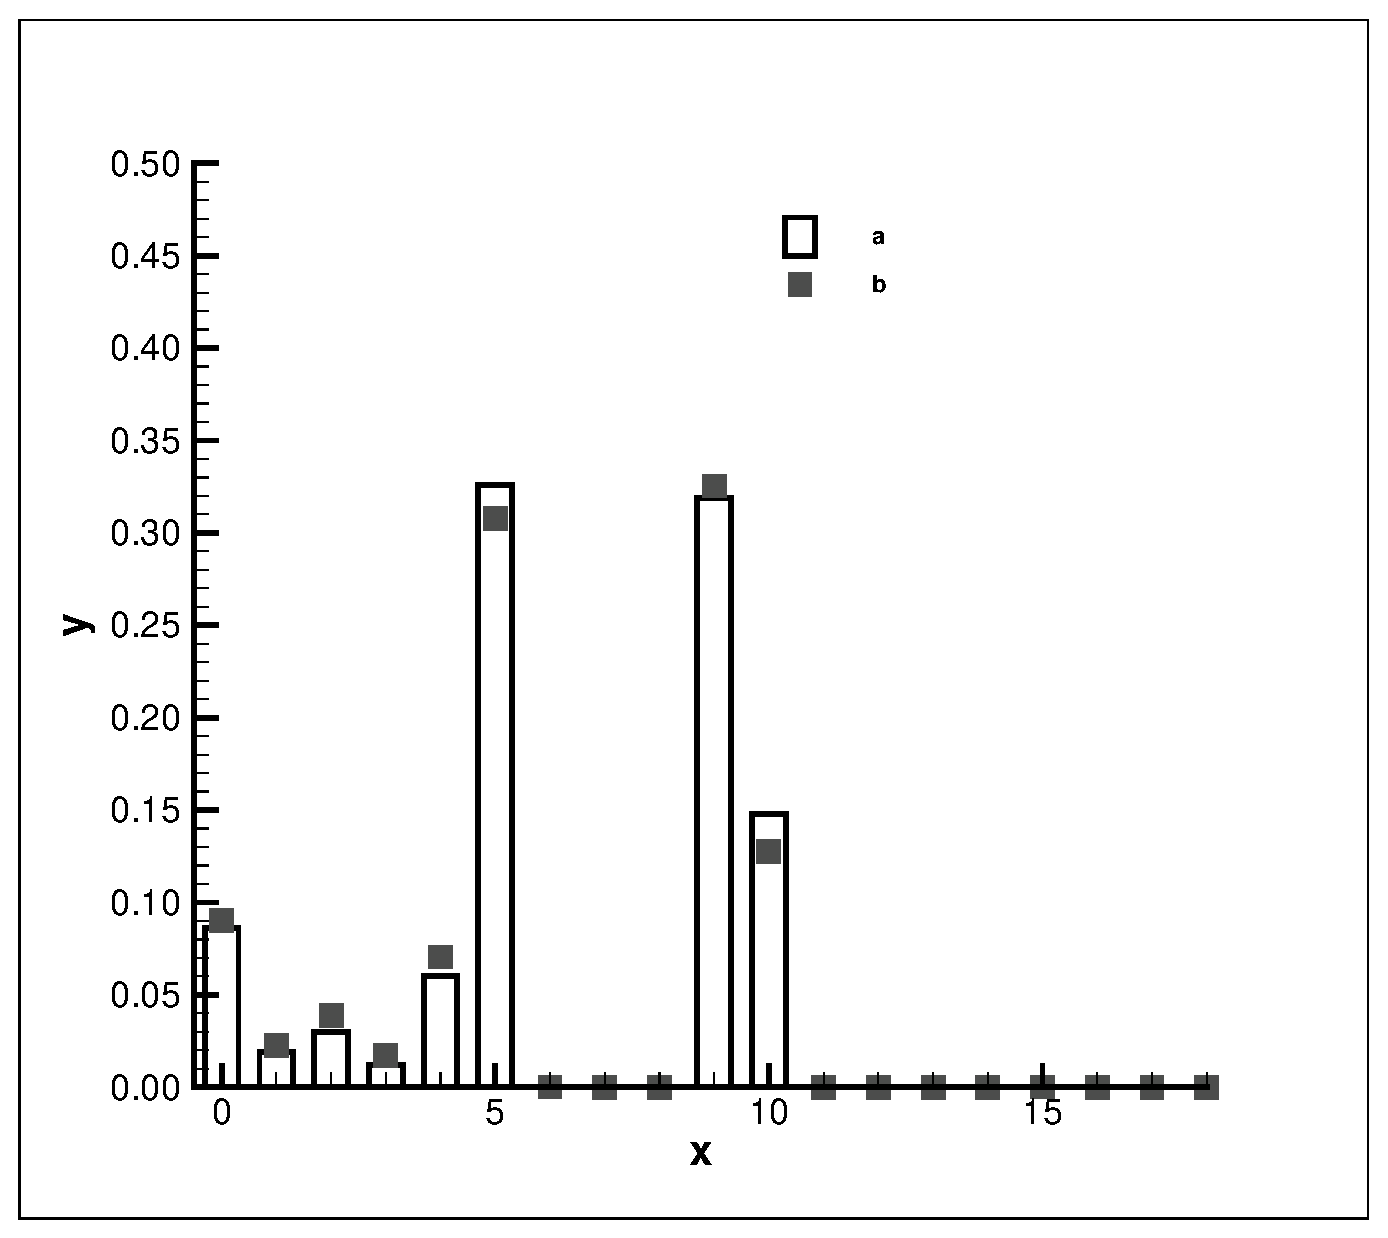
\includegraphics[width=8cm]{kero_oxycomprp1.eps}
% One can specify [angle=x,width=y,height=z] for the graphics
\caption{Equilibrium combustion results at an equivalence ratio of 1.33 for RP1, $\phi CH_2 + 1.5O_2 \to
H_2O + CO_2$
(taken from Hill and Peterson)}
\label{fig:rp1comp}
\end{center}
\end{figure}

	This result is seen with
other hydrocarbon fuels as well, as shown in Fig. \ref{fig:rp1comp}.  Here, the results (taken from
Hill and Peterson) of an equilibrium combustion calculation are shown for RP1 ($CH_{1.96}$) which
has approximately the same ratio of carbon to hydrogen as kerosene ($C_{12}H_{24}$).  These
results are for an equivalence ratio of 1.33 (which is approximately the equivalence ratio at which the 
peak equilibrium temperature is reached, see Fig. \ref{fig:kero_oxy}(A)) with an initial temperature 
and pressure of 298 K and 6.89 MPa respectively.  As can be seen, the combustion of kerosene at the same 
conditions matches the results for RP1, with the \emph{mole fraction} (as opposed to mass fraction as 
used in Fig. \ref{fig:kero_oxy} (B)) of $CO_2$ being significantly depleted, $CO$ amounts being elevated, and
residual $O_2$ being present despite the fact that the mixture is fuel rich.

	Going back to the conditions for which the results in Fig. \ref{fig:kero_oxy}(B) are obtained,
Fig. \ref{fig:kero_oxy_multiphi} shows the mass fractions of the various species over an 
increasing range of equivalence ratios, from a fuel lean mixture of $\phi = 0.5$ to a fuel
rich mixture with $\phi = 4.5$.  As can be seen, the mass fraction distribution at $\phi = 3$ 
exhibits a change in composition, from four species to two, as the decreasing amounts of both water
and carbon dioxide have finally reached zero leaving only hydrogen and carbon monoxide.  However
past this point at an equivalence ratio of 3.5, there are again four species, only this time the
new species are those arising out of the partial oxidization of kerosene, i.e., 
the kerosene is only partly broken down leaving some lighter unburned hydrocarbons behind such as
$C_2H_2$ and $C_2H_4$.  This sharp change in mixture composition, not merely changing the amounts of
given species, but actually changing the species present in the mixture, is responsible for the
sharp change in $\gamma$ seen in Fig. \ref{fig:kero_oxy}(A) at an equivalence ratio of 3.


\begin{figure}[hp]
\begin{center}
\psfrag{y}[c][c][0.7][0]{Mass Fraction ($c_i$)}
\psfrag{x}[c][c][0.7][0]{Species}
\subfigure[$\phi=0.5$]{
\includegraphics[width=5cm]{kero_oxy_phi0.5.eps}}
\subfigure[$\phi=1.0$]{
\includegraphics[width=5cm]{kero_oxy_phi1.0.eps}}
\subfigure[$\phi=1.5$]{
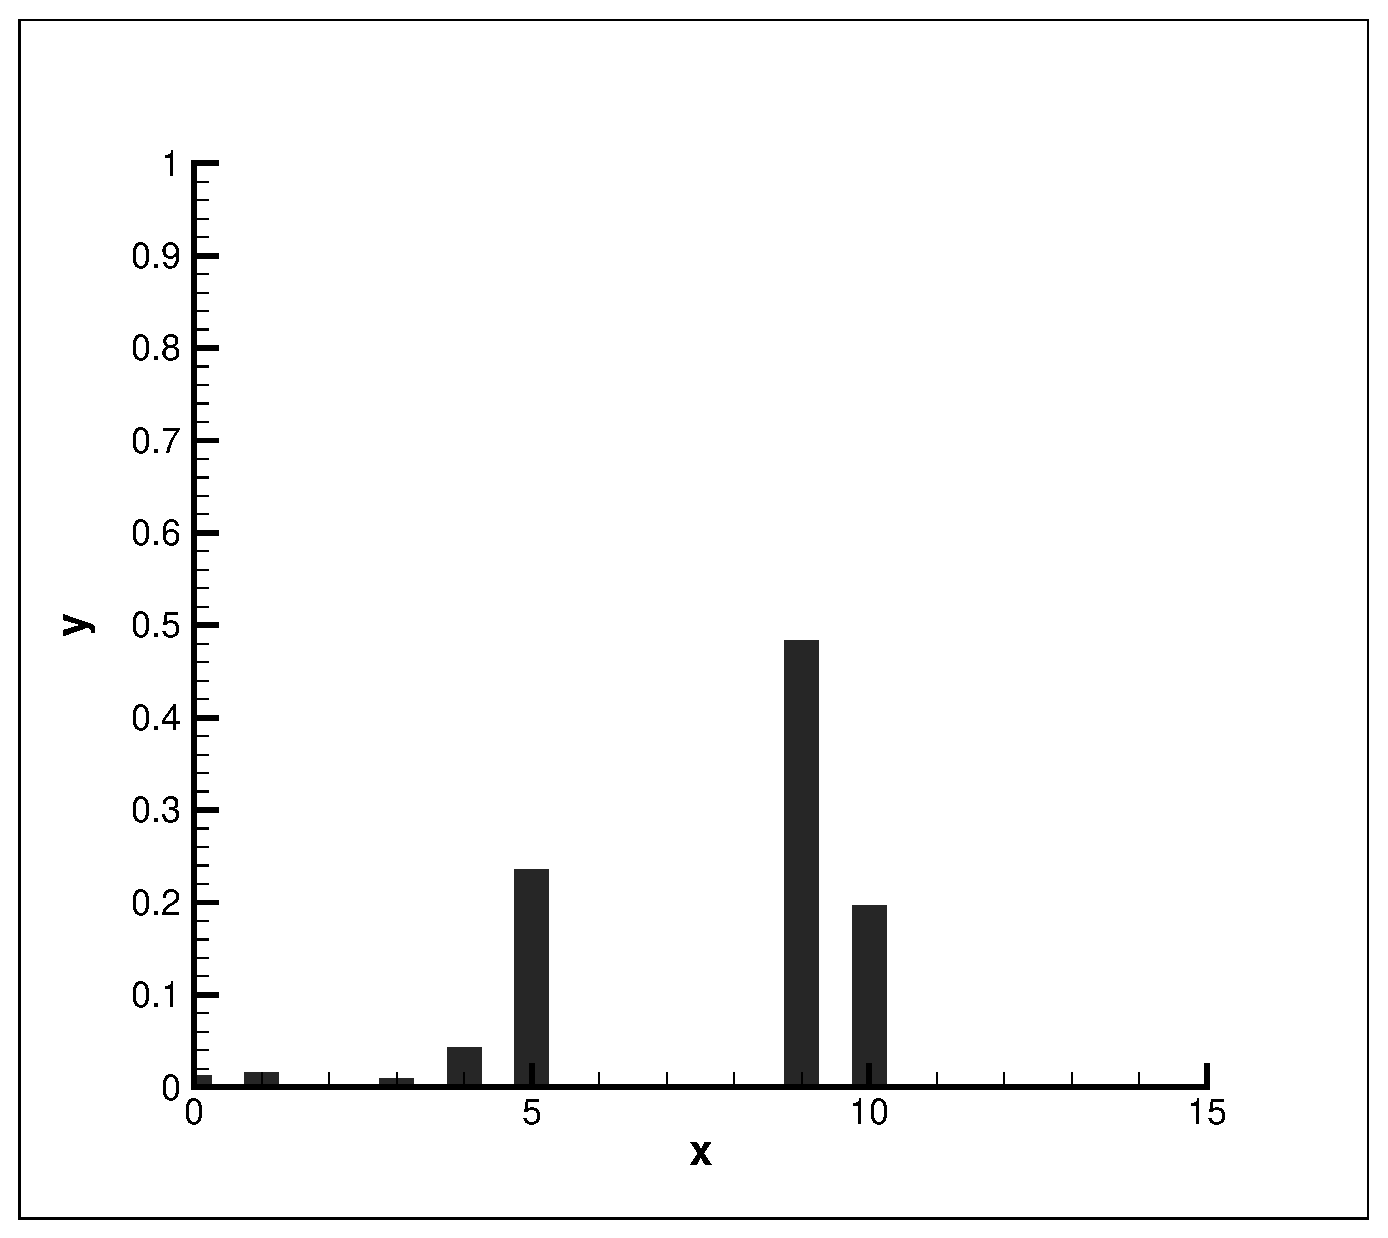
\includegraphics[width=5cm]{kero_oxy_phi1.5.eps}}
\subfigure[$\phi=2.0$]{
\includegraphics[width=5cm]{kero_oxy_phi2.0.eps}}
\subfigure[$\phi=2.5$]{
\includegraphics[width=5cm]{kero_oxy_phi2.5.eps}}
\subfigure[$\phi=3.0$]{
\includegraphics[width=5cm]{kero_oxy_phi3.0.eps}}
\subfigure[$\phi=3.5$]{
\includegraphics[width=5cm]{kero_oxy_phi3.5.eps}}
\subfigure[$\phi=4.0$]{
\includegraphics[width=5cm]{kero_oxy_phi4.0.eps}}
\subfigure[$\phi=4.5$]{
\includegraphics[width=5cm]{kero_oxy_phi4.5.eps}}

% One can specify [angle=x,width=y,height=z] for the graphics
\caption{Equilibrium combustion mass fractions at various equivalence ratios for kerosene/oxygen 
($T_{inj} = 300$ K, $p^o = 1.5$ MPa)}
\label{fig:kero_oxy_multiphi}
\end{center}
\end{figure}   

	To summarize, the presence of residual $O_2$ at equivalence ratios of less than 3 and greater than
1 does not indicate a fuel lean mixture, but rather that the combustion process represented by 
Eq. \ref{eqn:kerocombo2} is no longer valid (as partial dissociation of the combustion products occurs
due to the elevated temperature).  Also, if one assumes that the combustion process occurs as
follows (where the combustion products are now $CO$ and $H_2$),

\begin{equation}
	\phi C_{12}H_{24} + 6 O_2 \longrightarrow 12 CO + 12 H_2
\label{eqn:kerocombo2coh}
\end{equation}	

	then the ($\frac{f}{a}$) is 1/6 or 0.1667 on a molar basis or 0.8767 on a mass basis.  
Given molecular weights of 28.0104 kg/kmol and 2.01588 kg/kmol for $CO$ and $H_2$ respectively this leads 
to mass fractions of 0.932 for $CO$ and 0.067 for $H_2$ assuming Eq. \ref{eqn:kerocombo2coh}.  These
are indeed the values in Fig. \ref{fig:kero_oxy_multiphi}(F).  And comparing this fuel to air (or 
oxygen in this case) ratio to the stoichiometric value determined from Eq. \ref{eqn:kerocombo2} of 0.2916 
one realizes that $\frac{f}{a} = 0.8767$ is indeed 3 times this value, therefore $\phi = 3$.  
Thus at equivalence ratios higher than 3, the complete combustion model of Eq. \ref{eqn:kerocombo2} is
totally inaccurate and must be replaced with Eq. \ref{eqn:kerocombo2coh}.
%---------------------------------------------------------------------------------------------
\subsection{Nozzle Design Results}

	The following nozzle designs are for a combustion mixture of kerosene
($C_{12}H_{24}$) and pure oxygen ($O_2$) at an equivalence ratio, $\phi$, of one (based on the 
complete combustion reaction in Eq. \ref{eqn:kerocombo2}),

\begin{displaymath}
	\phi C_{12}H_{24} + 18 O_2 \longrightarrow 12 H_2O + 12 CO_2
\label{eqn:kerocombo2b}
\end{displaymath}

	The combustion is assumed to occur at a constant pressure of 1.5 MPa while the total 
temperature at the end of the combustion process is assumed to be equal to the equilibrium 
combustion temperature.  For an input fuel temperature of 300 K this yields a total temperature 
of  3533.55 K.  The pertinent combustion variables are summarized in Table \ref{table:mixture} while
the resulting mixture composition on both a mass and mole fraction basis is shown in
Fig. \ref{fig:mixcomp}.  The equilibrium combustion calculations consider a total of sixteen
possible species as listed in Table \ref{table:speciesmap}.

\begin{table}[!h]
\fontsizetable
\begin{center}
\begin{threeparttable}

\tablecaption{Mixture Properties}

\begin{tabular}{cc}
\toprule
Chamber Conditions		&	Value \\
\midrule
Equivalence Ratio, $\phi$       &	1\\
Fuel Input Temperature		&	300 K\\
Total Pressure			&	1.5 MPa\\
Post Combustion Equilibrium Temperature		&	3533.55 K\\
Post Combustion Specific Heat Ratio, $\gamma$	&	1.2175998\\
Post Combustion Mixture Molecular Weight	&	24.412 kg/kmol\\

\bottomrule
\end{tabular}

%\begin{tablenotes}
%\end{tablenotes}

\label{table:mixture}
\end{threeparttable}
\end{center}
\end{table}

\begin{table}[!h]
\fontsizetable
\begin{center}
\begin{threeparttable}

\tablecaption{Nozzle Design Parameters}

\begin{tabular}{cc}
\toprule
Nozzle Design Variable	&	Value \\
\midrule
Maximum Expansion Angle, $\omega$	&	$10^o$\\
Throat Radius				&	1 cm\\
Exit Mach Number, $M_e$			&	3, 4, 5\\
Wall Temperature			&	800 K\\
Mach Number at Combustion Chamber Exit 	&	0.1 \\
Subsonic Section Length (\% of Supersonic Length)&	25\% \\

\bottomrule
\end{tabular}

%\begin{tablenotes}
%\end{tablenotes}

\label{table:nozcomp}
\end{threeparttable}
\end{center}
\end{table}

\begin{table}[!h]
\fontsizetable
\begin{center}
\begin{threeparttable}

\tablecaption{Species Map for Figure \ref{fig:mixcomp}}

\begin{tabular}{cccccccccccccccc}
\toprule
0 & 1 & 2 & 3 & 4 & 5 & 6 & 7 & 8\\
\midrule
$H_2$ & $O_2$ & $H$ & $O$ & $OH$ & $H_2O$ & $HO_2$ & $C_2H_2$ & $C_2H_4$\\ 

\midrule
9 & 10 & 11 & 12 & 13 & 14 & 15 & \\
\midrule
$CO$ & $CO_2$ & $CH_3$ & $CH_4$ & $H_2CO$ & $C_6H_{12}O$ & $C_{12}H_{24}$ & \\
\bottomrule
\end{tabular}

%\begin{tablenotes}
%\end{tablenotes}

\label{table:speciesmap}
\end{threeparttable}
\end{center}
\end{table}

\begin{figure}[!h]
\begin{center}
\psfrag{y}[c][c][0.7][0]{Mass Fraction ($c_i$)}
\psfrag{x}[c][c][0.7][0]{Species}
\subfigure[Mass Fractions]{
\includegraphics[width=5.5cm]{kero_o2_mass_phi1.eps}}
\psfrag{y}[c][c][0.7][0]{Mole Fraction ($\chi_i$)}
\subfigure[Mole Fractions]{
\includegraphics[width=5.5cm]{kero_o2_mole_phi1.eps}}

% One can specify [angle=x,width=y,height=z] for the graphics
\caption{Post combustion mixture composition entering nozzle}
\label{fig:mixcomp}
\end{center}
\end{figure}  

\begin{figure}[!hb]
\begin{center}

\psfrag{x}[c][c][0.7][0]{x [m]}
\psfrag{y}[c][c][0.7][0]{y [m]}
\psfrag{b}[l][c][0.5][0]{Inviscid Contour}
\psfrag{a}[l][c][0.5][0]{Final Contour}
\psfrag{c}[l][c][0.5][0]{Boundary Layer}
\subfigure[Inviscid contour and boundary layer for $M_e = 5$]{
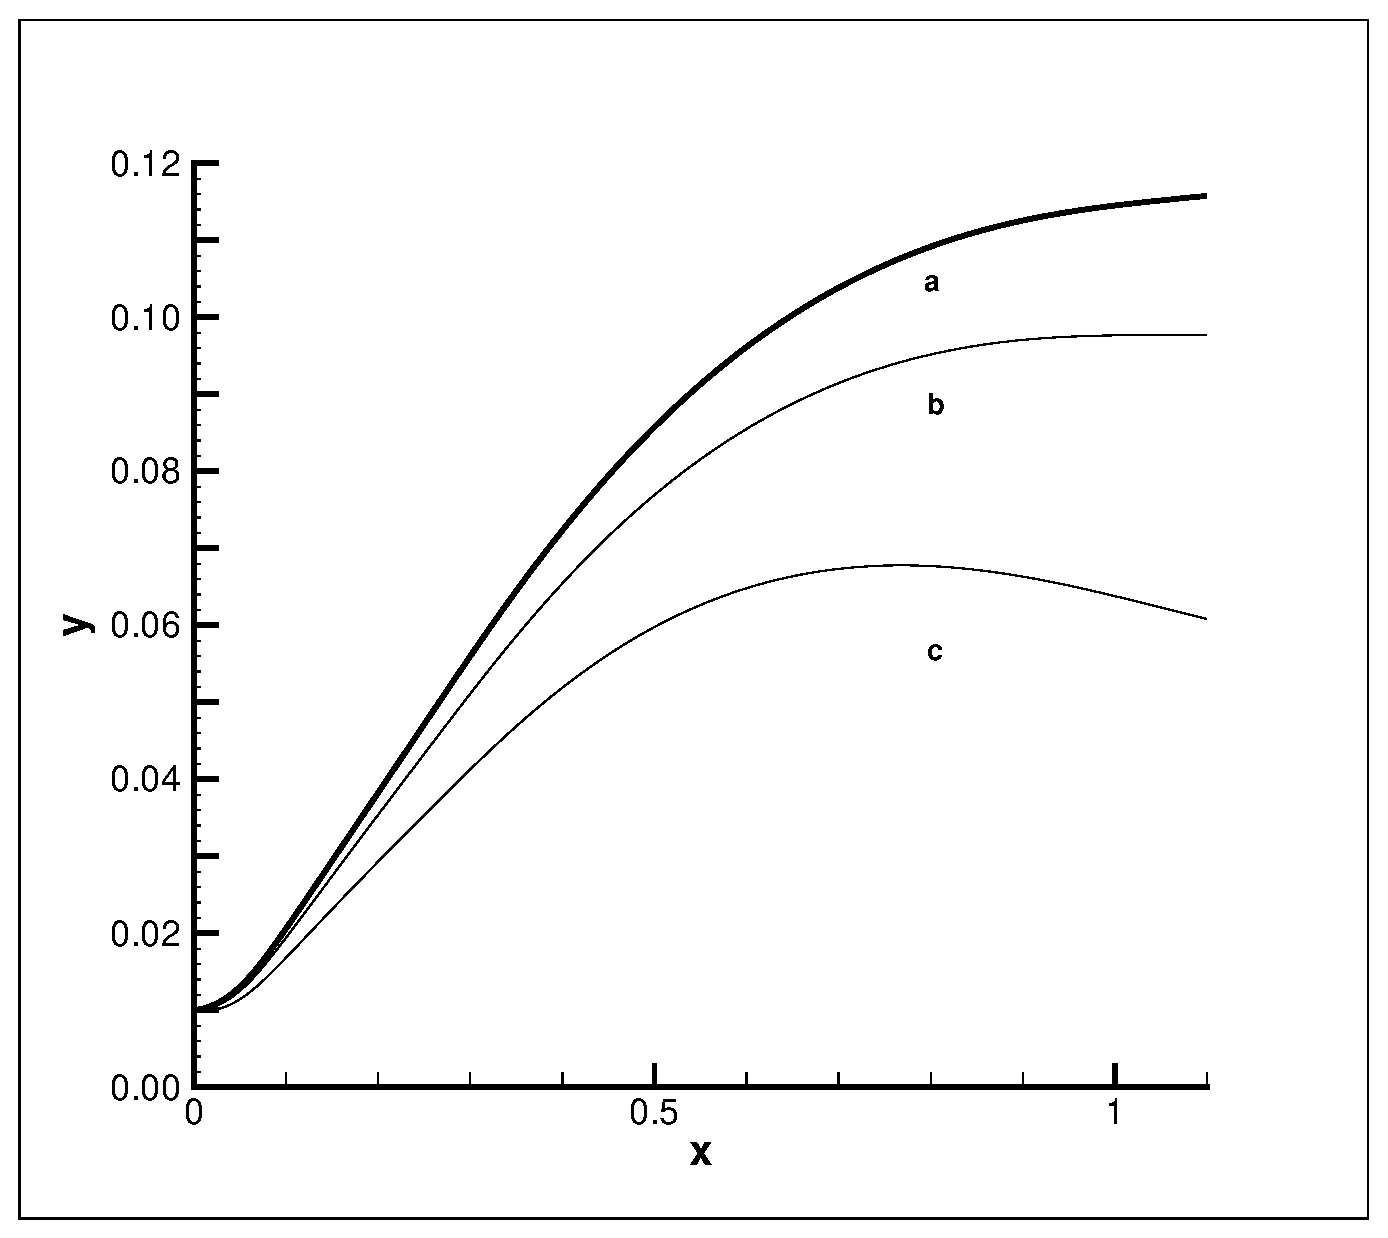
\includegraphics[width=5.5cm]{mach5inv.eps}}
\subfigure[Complete axisymmetric nozzle shape for $M_e = 5$]{
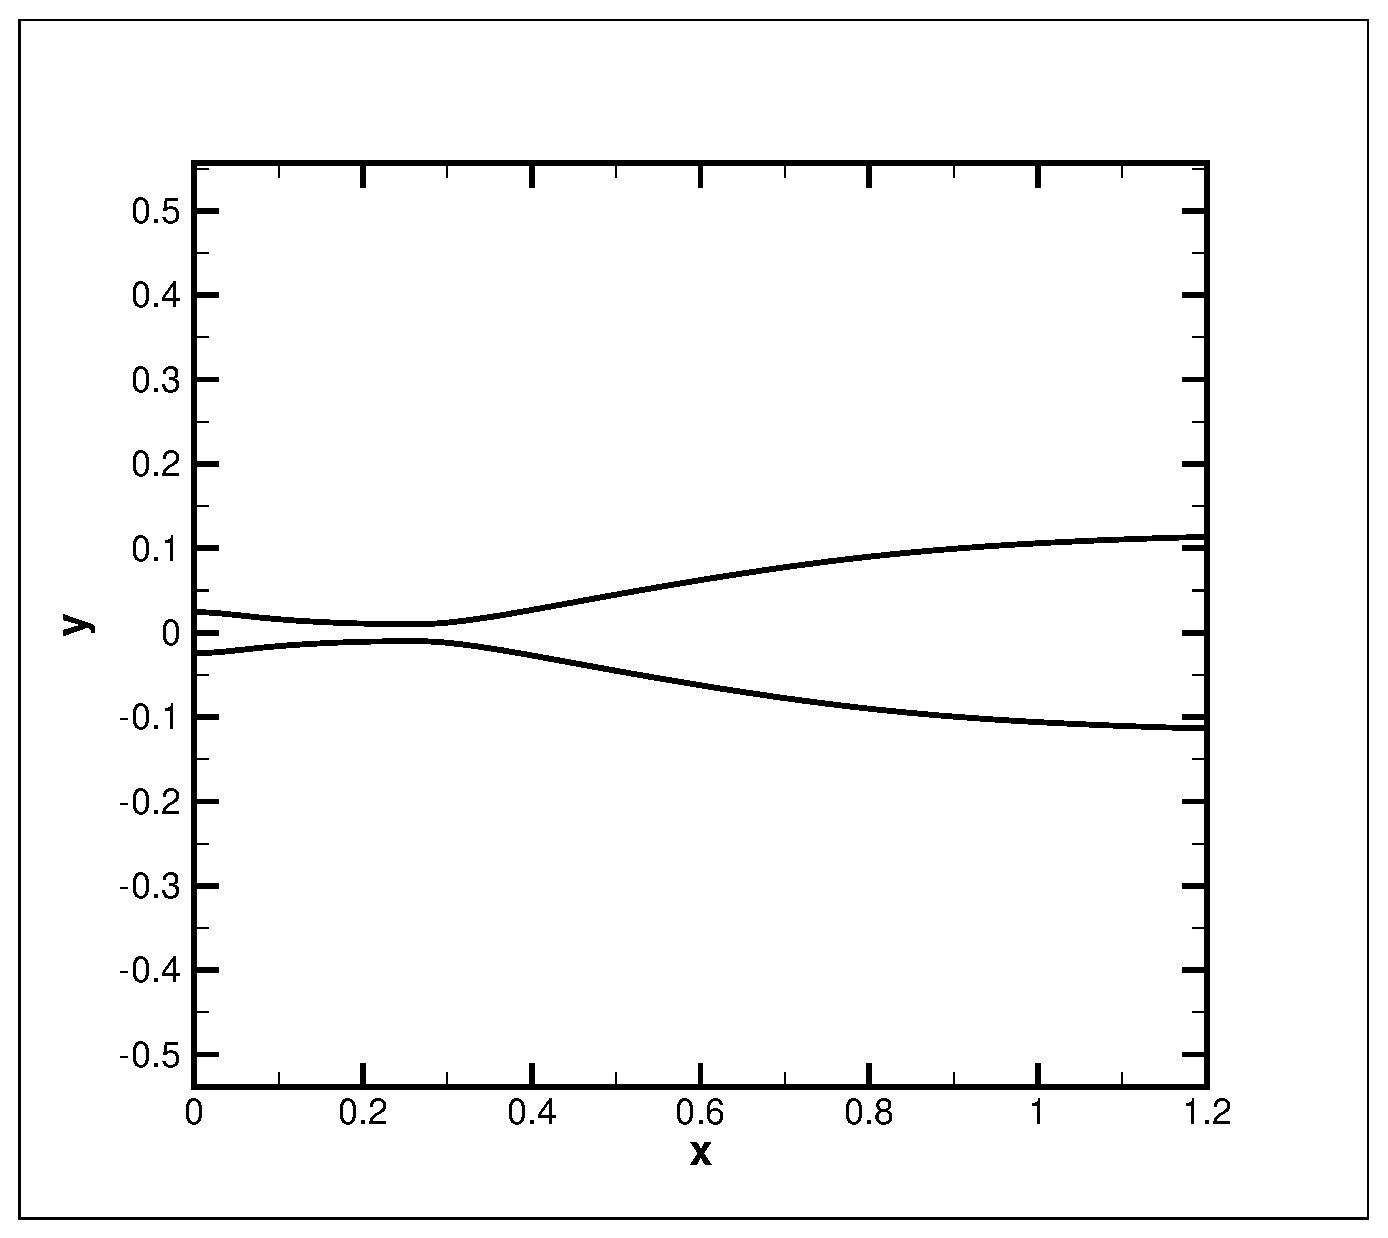
\includegraphics[width=5.5cm]{scalewholenozzle.eps}}
\caption{Axisymmetric Nozzle Design}
\label{fig:inviscid}
\end{center}
\end{figure}

\begin{figure}[ht]
\begin{center}
\psfrag{c}[l][c][0.65][0]{$M_e = 3$}
\psfrag{b}[l][c][0.65][0]{$M_e = 4$}
\psfrag{a}[l][c][0.65][0]{$M_e = 5$}
\psfrag{x}[c][c][0.7][0]{x [m]}
\psfrag{y}[c][c][0.7][0]{y [m]}

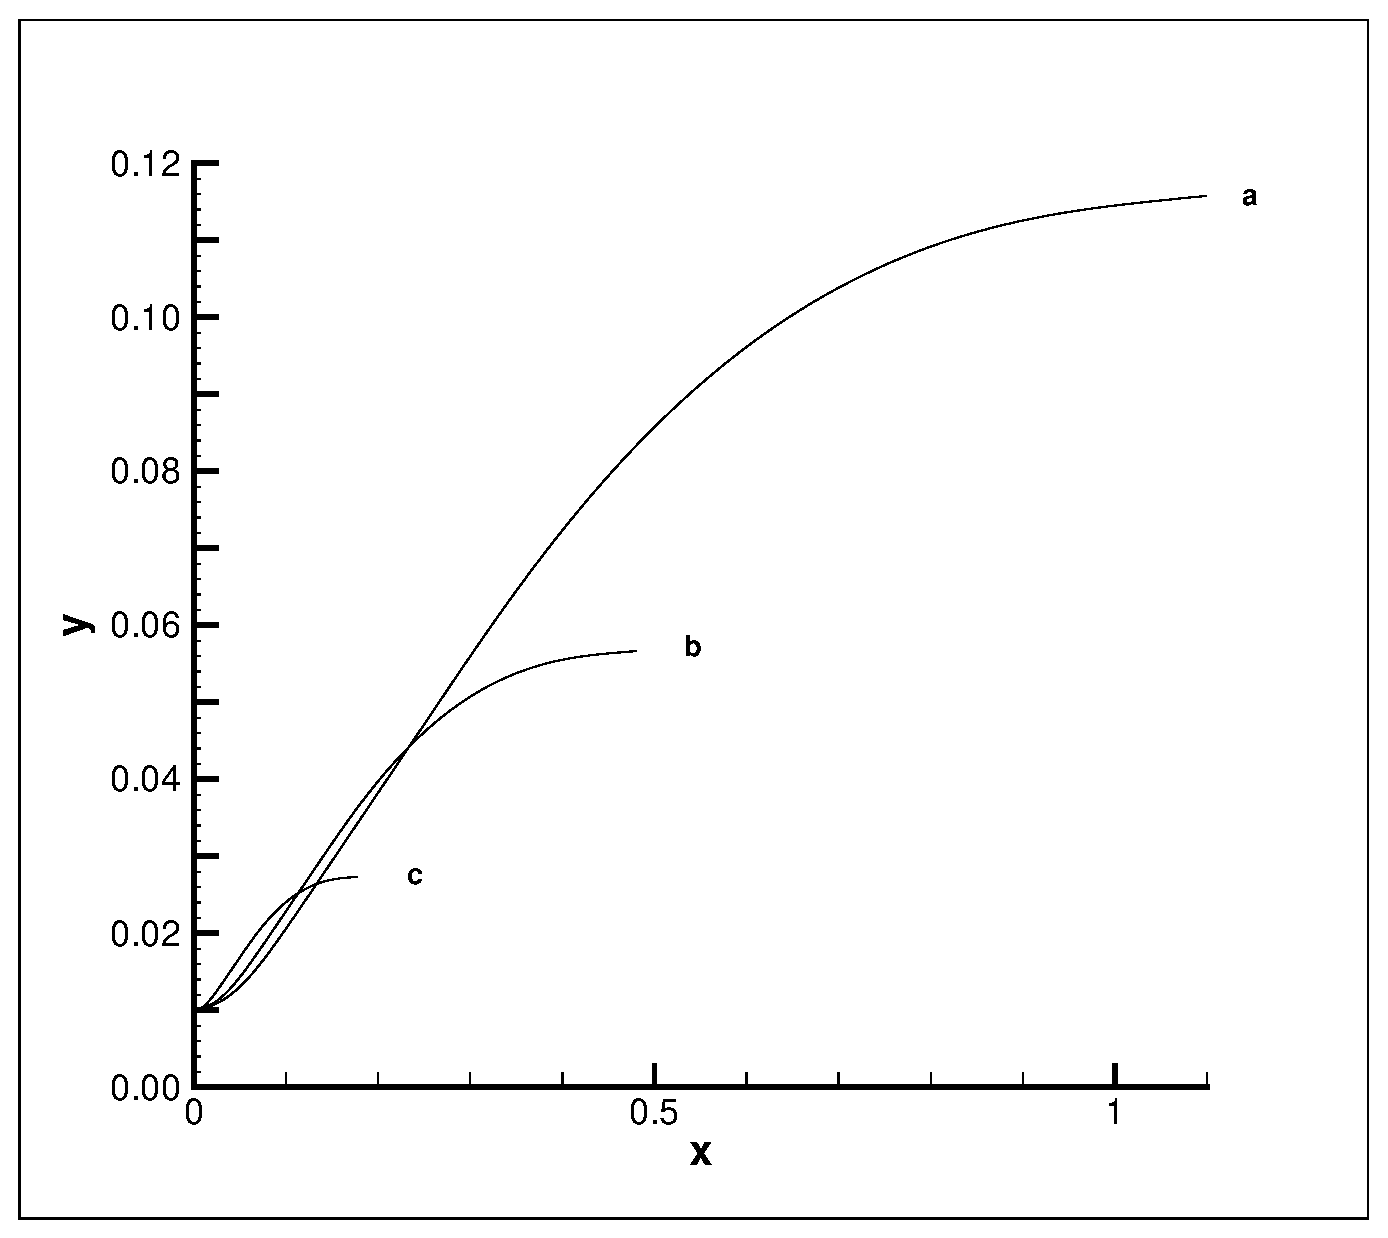
\includegraphics[width=10cm]{nozcomp.eps}
\caption{Nozzle designs for various exit Mach numbers}
\label{fig:contcomp}
\end{center}
\end{figure}

	For an exit Mach number of 5, Fig. \ref{fig:inviscid}(A) shows the inviscid contour
created and the resulting final contour after being adjusted for the presence of the boundary layer
(which is also shown in the figure).  As one can see, the resulting boundary layer at the 
nozzle exit is quite large which results in many cases in a truncation of the nozzle length to 
maximize the resulting high velocity core region.  Adding a subsonic portion ahead of the throat with a 
length set at 25\% of the diverging length and a chamber Mach number of 0.1 yields the nozzle shape 
shown in Fig. \ref{fig:inviscid}(B).  Various nozzle designs are shown in Fig. \ref{fig:contcomp} for 
nozzles with several different exit Mach numbers (while all other input variables remain constant). 

%---------------------------------------------------------------------------------------------------------
\subsection{Computational Results}

	The preceding nozzle design is used in an axisymmetric, implicit, steady state computational code 
(which uses the Wilcox $k-\omega$ two equation turbulence model) to verify the predictions made (this
code is called WARP, developed by B. Parent).  
A uniform grid with 150 points in the downstream direction (parallel to the nozzle axis) and 50 points
in the cross stream direction is used.  Figure \ref{fig:warpcent} shows the Mach number along the nozzle 
centreline as compared to both the desired Mach number distribution (as found from the method previously
described) and the isentropic area/mach number relation (Eq. \ref{eqn:area}).

\begin{figure}[!h]
\begin{center}
\psfrag{y}[c][c][0.7][0]{Mach Number}
\psfrag{x}[c][c][0.7][0]{Distance along Centreline [m]}
\psfrag{a}[l][c][0.5][0]{Computational Result (150 x 50 Grid)}
\psfrag{b}[l][c][0.5][0]{Pre-specified Mach Number Distribution}
\psfrag{c}[l][c][0.5][0]{Isentropic Mach Number Distribution (Eq \ref{eqn:area})}
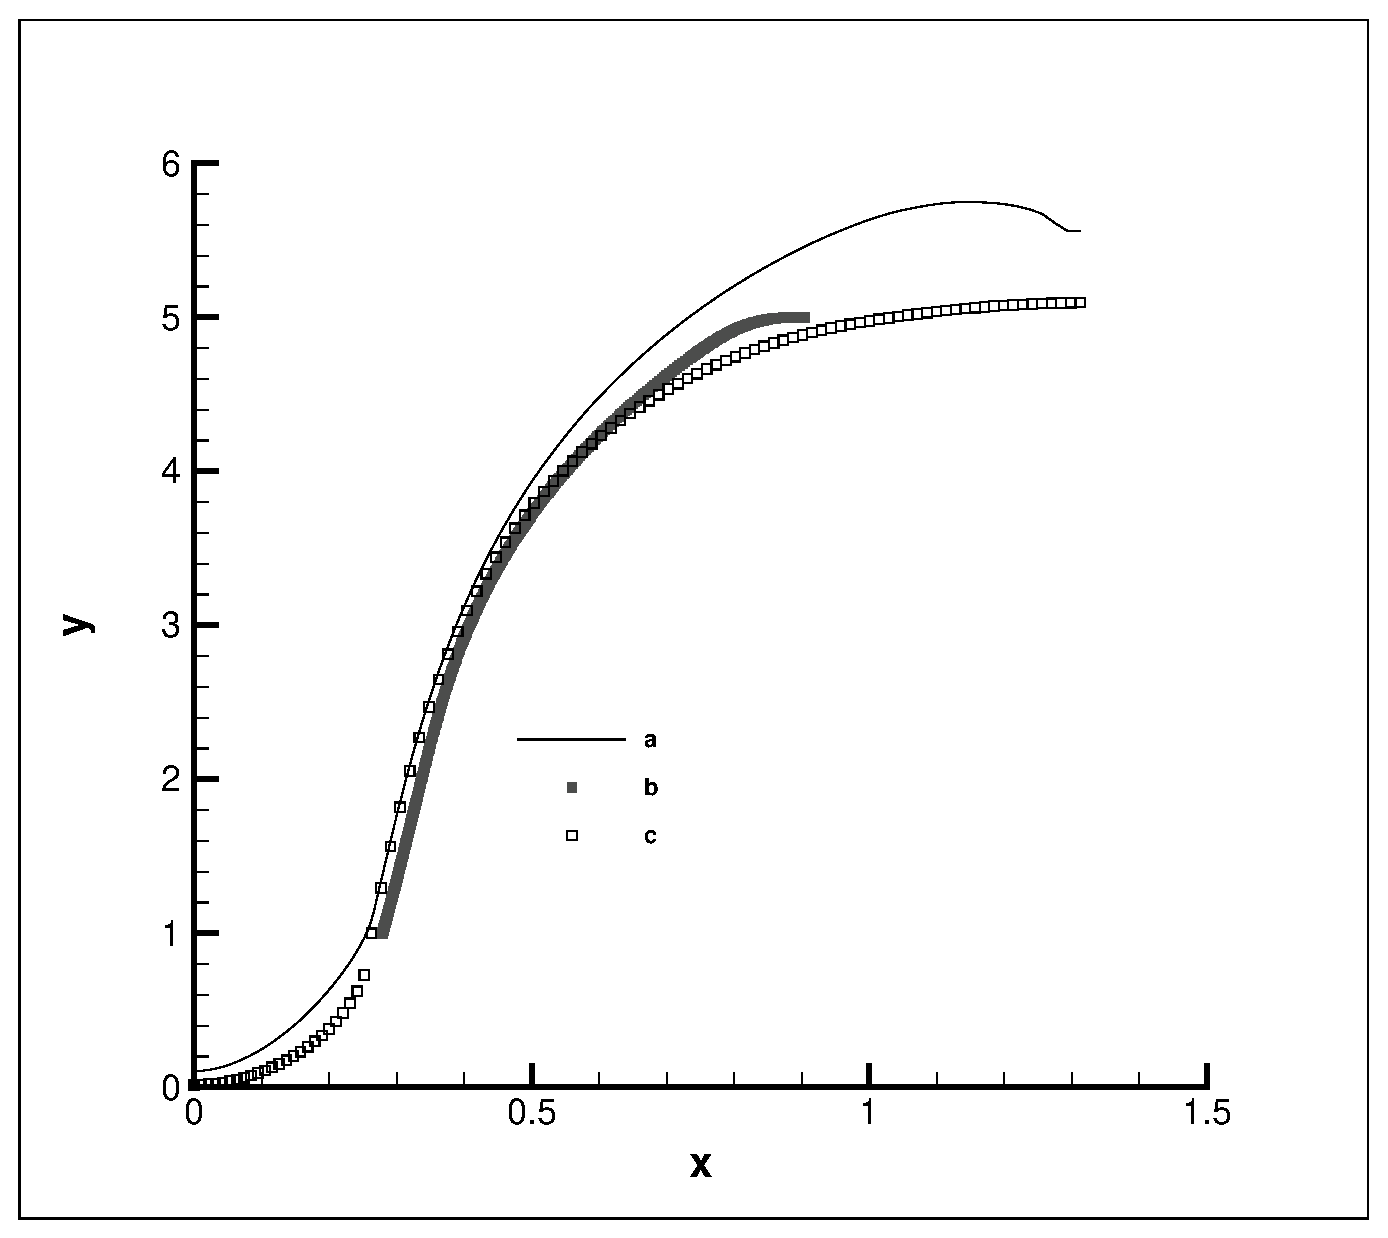
\includegraphics[width=9cm]{warpcentcomp.eps}
% One can specify [angle=x,width=y,height=z] for the graphics
\caption{Mach number along nozzle centreline}
\label{fig:warpcent}
\end{center}
\end{figure}  

	As can be seen, although the computed Mach number at the exit of approximately 5.6 is slightly higher 
than the design Mach number of 5, it does follow the desired contour as the velocity is increased from 
Mach one at the throat through the expanding portion of the nozzle.  In fact, as can be seen up to a  
distance of approximately 0.5 m, the predicted increase in Mach number follows the desired increase 
quite well.  It is also noted that the pre-specified Mach number distribution also follows the isentropic
relation very closely, which is to be expected given the manner in which the nozzle is designed.  In using
the two dimensional method of characteristics for irrotational flow, from Crocco's theorem one can conclude
that since the conditions at the end of the combustion chamber are assumed uniform (i.e. constant enthalpy
everywhere) then the flow must be homentropic (constant entropy everywhere).  If the flow is homentropic, then
it must also be isentropic (entropy is constant along a given streamline, but not necessarily constant 
\emph{between} streamlines) and hence Eq. \ref{eqn:area} must apply.

\begin{figure}[p]
\begin{center}
\psfrag{y}[c][c][0.7][0]{$\gamma$[m]}
\psfrag{x}[c][c][0.7][0]{x[m]}
\psfrag{z}[c][c][0.7][0]{Temperature [K]}
\psfrag{a}[l][c][0.5][0]{Nozzle Contour}
\psfrag{b}[l][c][0.5][0]{Computed $\gamma$}
\psfrag{c}[l][c][0.5][0]{Computed Temperature}
\psfrag{d}[l][c][0.5][0]{Isentropic Temperature}
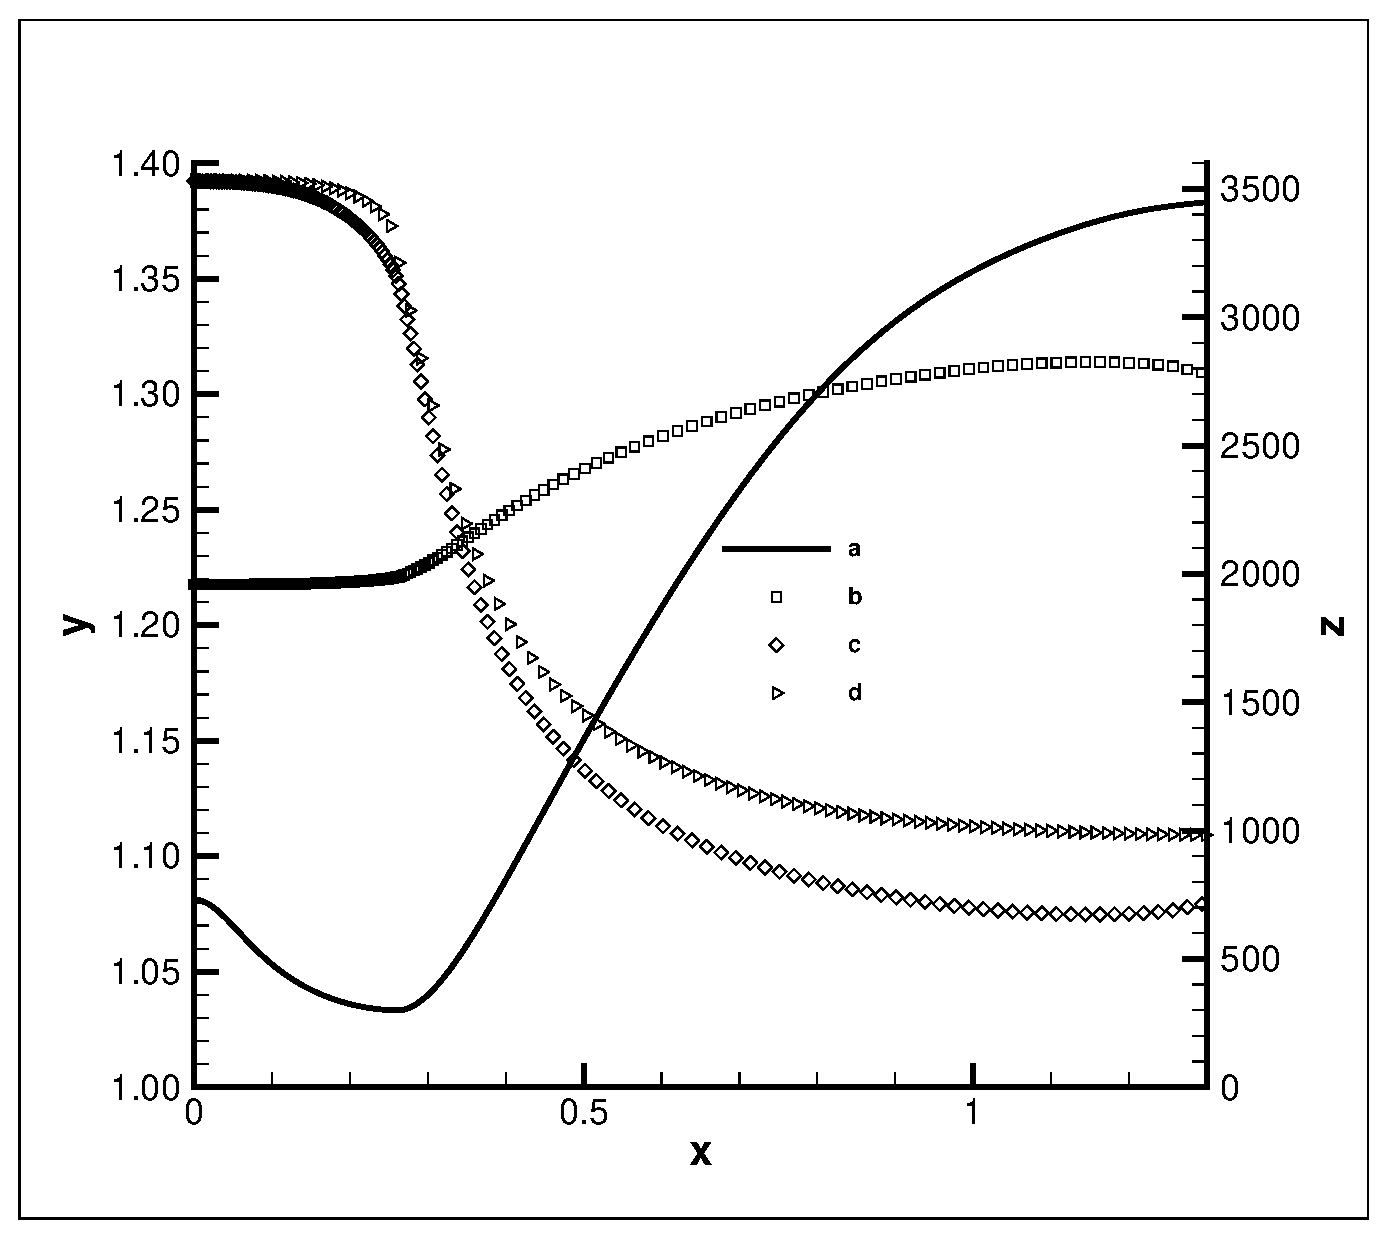
\includegraphics[width=9cm]{warpgamma.eps}
% One can specify [angle=x,width=y,height=z] for the graphics
\caption{Variation of Temperature and Specific Heat Ratio along Nozzle Centreline}
\label{fig:warpgamma}
\end{center}
\end{figure}

	The slight decrease in Mach number in the computational solution near the nozzle exit is caused 
by an increase in temperature at this location, as can be seen in Fig. \ref{fig:warpgamma}.  
Near the nozzle exit, the slope of the wall is nearly parallel with the nozzle axis and is thus approximately
a constant area duct.  Viscous effects in a constant area duct cause the temperature to rise and the Mach number
to tend to unity, thereby causing the decrease in Mach number and the increase in temperature seen at this
location.  Also shown in Fig. \ref{fig:warpgamma} is the isentropic temperature relation which follows the computed solution
very well until approximately the 0.4 m location, at which point the real gas effects become significant thereby
reducing the accuracy of assuming isentropic flow.  It is also noted that the isentropic result shows no temperature
increase at the nozzle exit, reinforcing the fact that the computed temperature rise is indeed a viscous 
effect.  

\begin{figure}[p]
\begin{center}
\psfrag{y}[c][c][0.7][0]{y[m]}
\psfrag{x}[c][c][0.7][0]{x[m]}
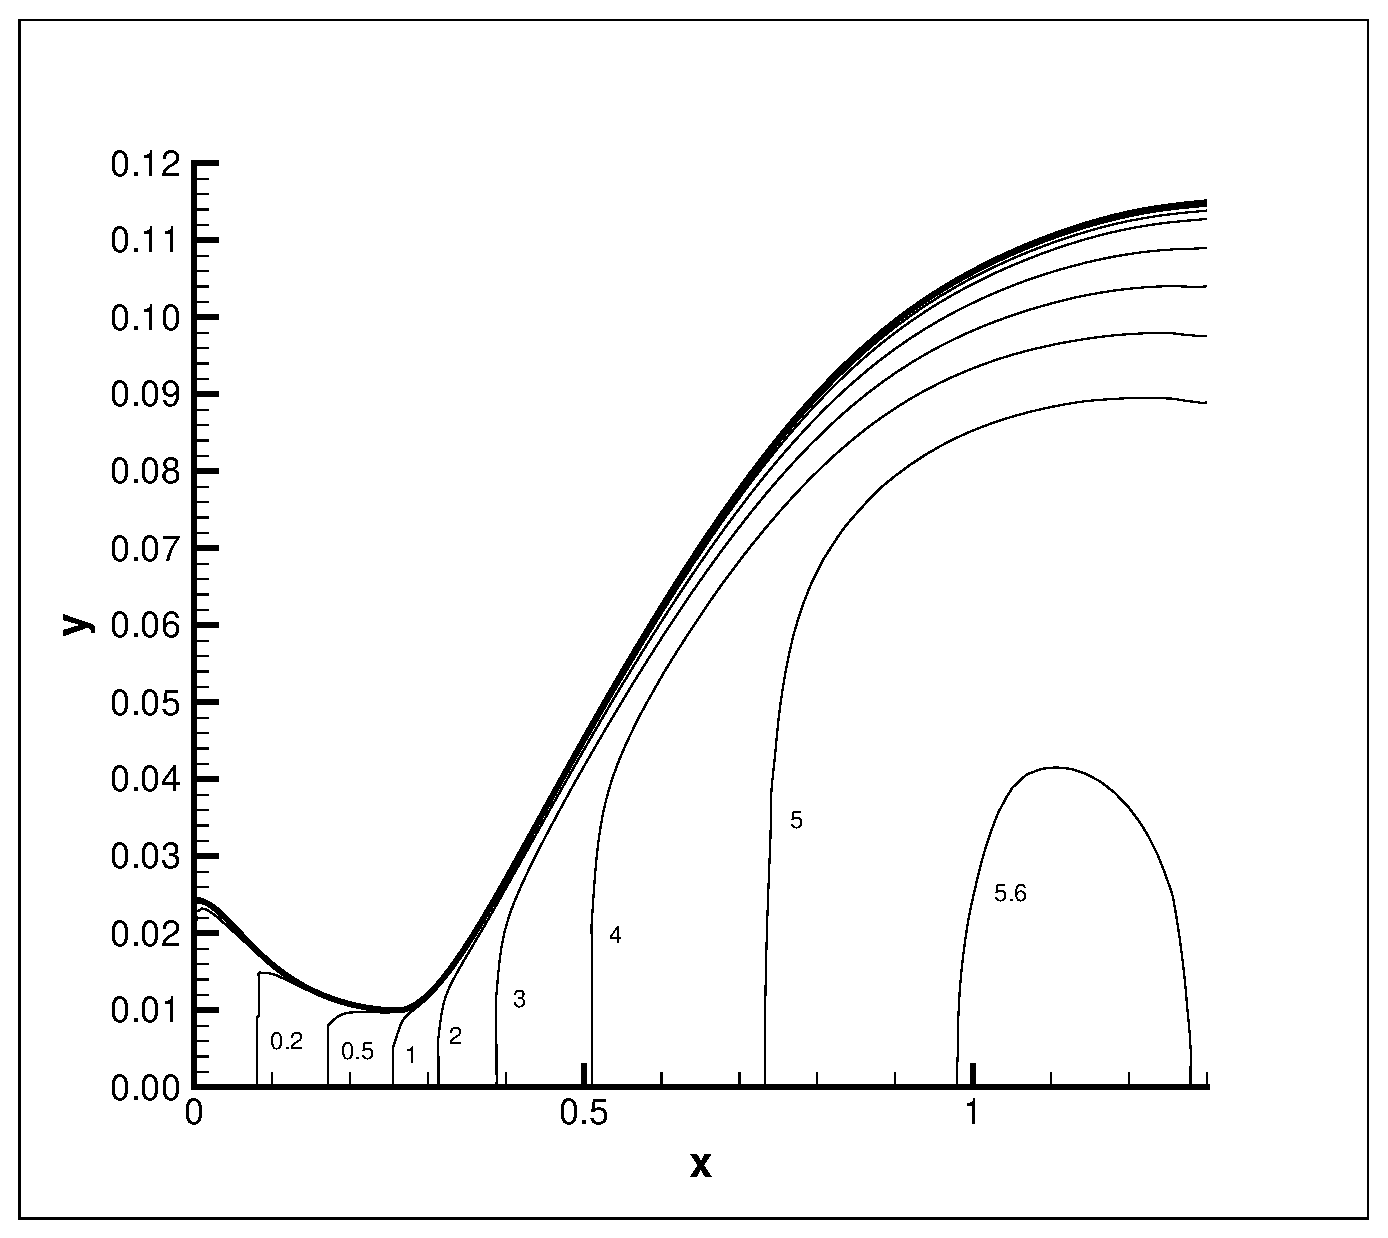
\includegraphics[width=9cm]{warpmachcont.eps}
% One can specify [angle=x,width=y,height=z] for the graphics
\caption{Mach contours within nozzle}
\label{fig:warpmach}
\end{center}
\end{figure}

	Also shown in Fig. \ref{fig:warpgamma} is the value for the ratio of specific heats throughout
the nozzle.  At the combustion chamber exit it starts at the value found from the equilibrium combustion 
calculations.  During the nozzle design, this value is assumed constant throughout the expansion process and
as can be seen from the computational results, this assumption is fairly accurate within the subsonic
portion of the nozzle.  However, as the expansion process continues past 
a distance downstream of approximately 0.4 m (Fig. \ref{fig:warpgamma})
the constant $\gamma$ assumption starts to become less valid.  This accounts for the differences in the
computed mach number in the latter portions of the nozzle as compared to the pre-specified distribution.
This change in $\gamma$ is also responsible for the difference between the pre-specified and isentropic Mach
number and temperature distributions shown in Figs. \ref{fig:warpcent} and \ref{fig:warpgamma}, since for the isentropic results $\gamma$ is held
constant at the combustion chamber exit value (approximately 1.22).

	Figure \ref{fig:warpmach} shows the Mach contours in within the nozzle.  Here one can see the
approximate shape of the boundary layer (as these contours depend on velocity \emph{and} temperature, hence
although the decreasing velocity is shown in the Mach number contours near the wall, this decrease is altered
to some extent by the increasing temperature as one approaches the wall as well).  Also, one can see the 
bubble of increased velocity along the nozzle centreline above the design Mach number of 5.  




% LocalWords:  Subsonic Dalton's kmols kmol
